% =======================================
%
% Verwendete zusätzliche Pakete
%
% =======================================


% Vorlesungsbezeichnungen setzen
\setvalue{vorlesungsnummer}{WS2020}
\setvalue{vorlesungsbezeichnung}{BBAF-VZ/BB}
\setvalue{author}{Wolfgang Murth, Martin Nigitsch}
 
 
% Setzen der Dokumenteninformationen für die PDF Datei
\setvalue{pdfauthor}{\getvalue{author}}
\iftoggle{german}
{
	\setvalue{pdftitle}{Excel Funktionen, Grundlagen Wirtschaftsinformatik (WS2020)}
}
{
	\setvalue{pdftitle}{Excel Funktionen, Grundlagen Wirtschaftsinformatik (WS2020)}
}
\setvalue{pdfsubject}{ }
\setvalue{pdfkeywords} {}
\setvalue{pdfcreationdate}{20200901120000}
\setvalue{pdfmoddate}{20200901120000}
% Übernehmen der Variablen für das PDF
\setpdfinfo

\renewmenumacro{\menu}{roundedmenus}

% =======================================
%
% Dokumentenbeginn
%
% =======================================

\begin{document}
 
% Fußzeile links (DEFAULT: Vorlesungsbezeichnung)
%\footerleft{\vorlesungsbezeichnung} 
 
% Fußzeile rechts (DEFAULT: Autor)
%\footerright{\getvalue{author}} 


% =======================================
%
% Deckblatt
%
% =======================================
\begin{titlepage}
\begin{textblock}{100}(0	,220)
\getvalue{author}\\

\vorlesungsbezeichnung  (\vorlesungsnummer)

\end{textblock}
\begin{textblock}{120}(22.5	,0)
	%\includegraphics[width=8cm]{images/excel_toplogo2010}
\end{textblock}

	\vspace*{5.8cm}
	\begin{center}
		\Huge

\iftoggle{german}
{
	\textbf{Excel Funktionen\\\Large{\vspace{0.3cm}Grundlagen Wirtschaftsinformatik\\WS2020}}\\
}
{
	\textbf{Excel Funktionen\\Grundlagen Wirtschaftsinformatik\\WS2020}\\
}

		
		
		\normalsize
	\end{center}	
\end{titlepage}

% =======================================
%
% Inhaltsverzeichnisse
%
% =======================================
\tableofcontents
%\clearpage
\listoffigures
\listoftables
%\lstlistoflistings
\clearpage



%=============================================================================
%=============================================================================
%=============================================================================


\clearpage
\section{Datumsfunktionen}

\subsection{Allgemeines}

Für Excel beginnt die Zeitrechnung am 0.1.1900. Das klingt seltsam, hat aber seinen Ursprung in  einer längst vergessenen Software, nämlich dem Tabellenkalkulationsprogramm Lotus 123.
Dieses Programm hatte einen Bug, denn es sah das Jahr 1900 als Schaltjahr an, was aber nicht stimmt. Um mit dem damaligen Platzhirsch kompatibel zu sein, baute Microsoft absichtlich
diesen Fehler ein. Deswegen beginnt die Microsoftsche Zeitrechnung mit dem 0.1. und nicht mit dem 1.1., damit ab dem 1. März 1900 der Kalender wieder stimmt.

Für Excel ist jedes Datum eine Zahl, beginnend mit dem 0.1.1900 mit der Zahl 0. Der 1.1.1900 ist dann 1 und so weiter. Der 1.1.1950 ergibt demnach 18264 und der 11.11.2009 den Wert 40128. Sobald Sie nun eine Zelle als Datum formatieren, weiß Excel, dass es diese Zahl
in ein Datumsformat wandeln soll.
	\begin{figure}[H]
		\centering
			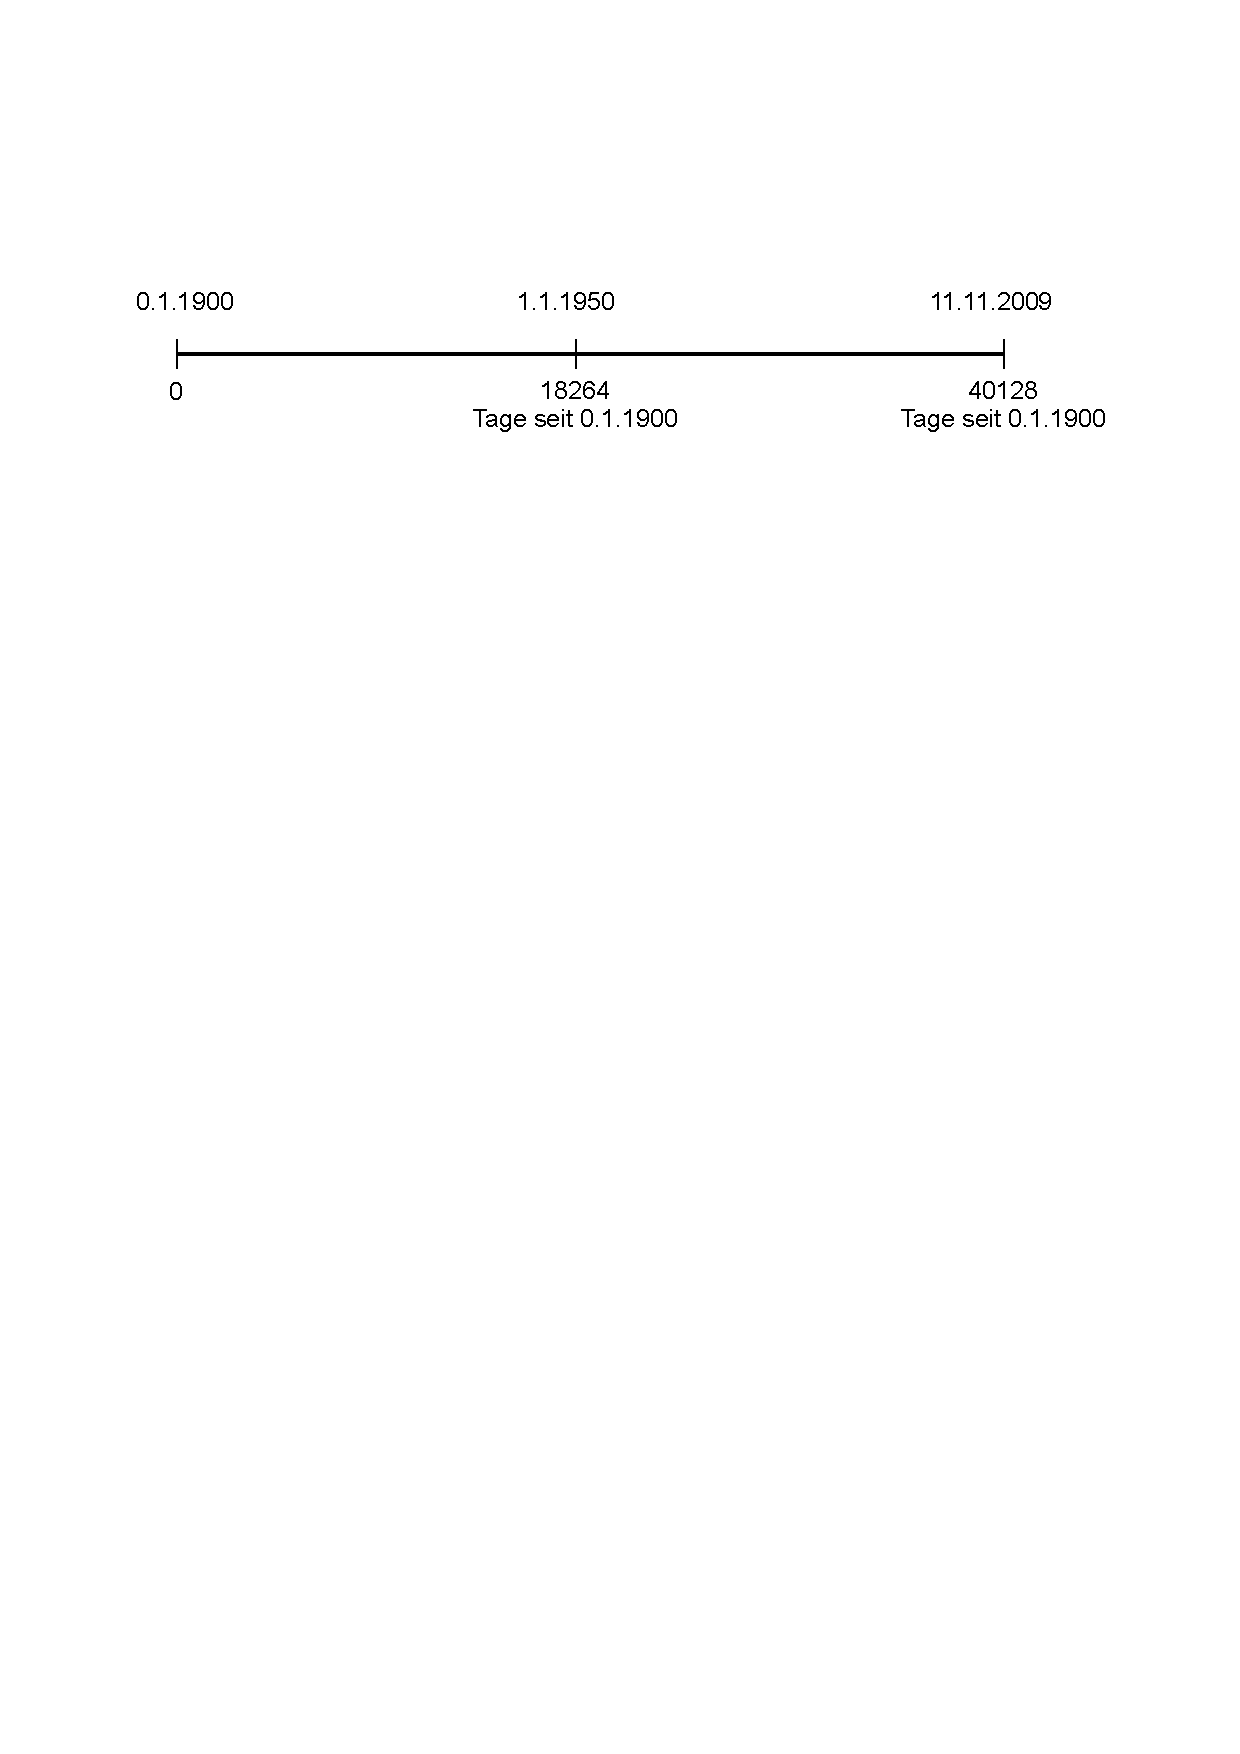
\includegraphics{_OpenOffice/datum.pdf}
		\caption{Datumsdarstelung in Excel}
		\label{fig:datum}
	\end{figure}

%\placefigure[middle,force][fig:datum]{}{\externalfigure[datum]}

Der Vorteil dieser Darstellung ist, dass man mit Daten einfach rechnen kann.
%\placefigure[middle,force][fig:datumdiff]{}{\externalfigure[datumdiff]}
	\begin{figure}[H]
		\centering
		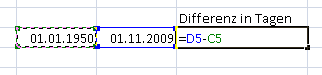
\includegraphics{images/datumdiff.png}
		\caption{Rechnen mit Datumsangaben}
		\label{fig:datumdiff}
	\end{figure}


Der Haken ist nur der, dass Excel in seiner grenzenlosen Intelligenz das Format der Quellzelle übernimmt, welche ein Datum ist. Dadurch erhalten sie nicht die Differenz in Tagen, sondern ein seltsames Datum.
%\placefigure[middle,force][fig:datumdiff2]{}{\externalfigure[datumdiff2]}
	\begin{figure}[H]
		\centering
		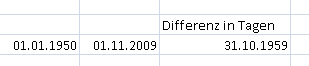
\includegraphics{images/datumdiff2.png}
		\caption{Formatfehler der Datumsberechnung}
		\label{fig:datumdiff2}
	\end{figure}




Sie müssen nun die Zelle auf das Format Standard oder Zahl ändern um das richtige Ergebnis anzuzeigen.
%\placefigure[middle,force][fig:datumdiff3]{}{\externalfigure[datumdiff3]}
	\begin{figure}[H]
		\centering
		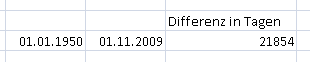
\includegraphics{images/datumdiff3.png}
		\caption{Tagesdifferenz als Zahl formatiert}
		\label{fig:datumdiff3}
	\end{figure}



%\placefigure[right,force][fig:alter1]{}{\externalfigure[alter1]}
	\begin{figure}[H]
		\centering
		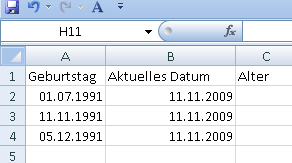
\includegraphics{images/alter1.png}
		\caption{Altersdifferenzen, Ausgangslage}
		\label{fig:alter1}

	\end{figure}


Berechnen wir nun als Beispiel das Alter von drei Freunden, welche alle im selben Jahr geboren wurden und zwar am 1.7.1991, am 11.11.1991 und am 5.12.1991. Der Zeitpunkt der Berechnung ist am Geburtstag des zweiten, also am
11.11.1991. Wir wissen, dass Excel ein Datum intern als Zahl behandelt. Dadurch kann man ein Datum vom anderen abziehen.

Erstellen wir nun die Berechnungformel Schritt für Schritt für den ältesten der drei Freunde, welcher am 1.7.1991 geboren wurde.
%\placefigure[middle,force][fig:datum2]{}{\externalfigure[datum2]}
	\begin{figure}[H]
		\centering
		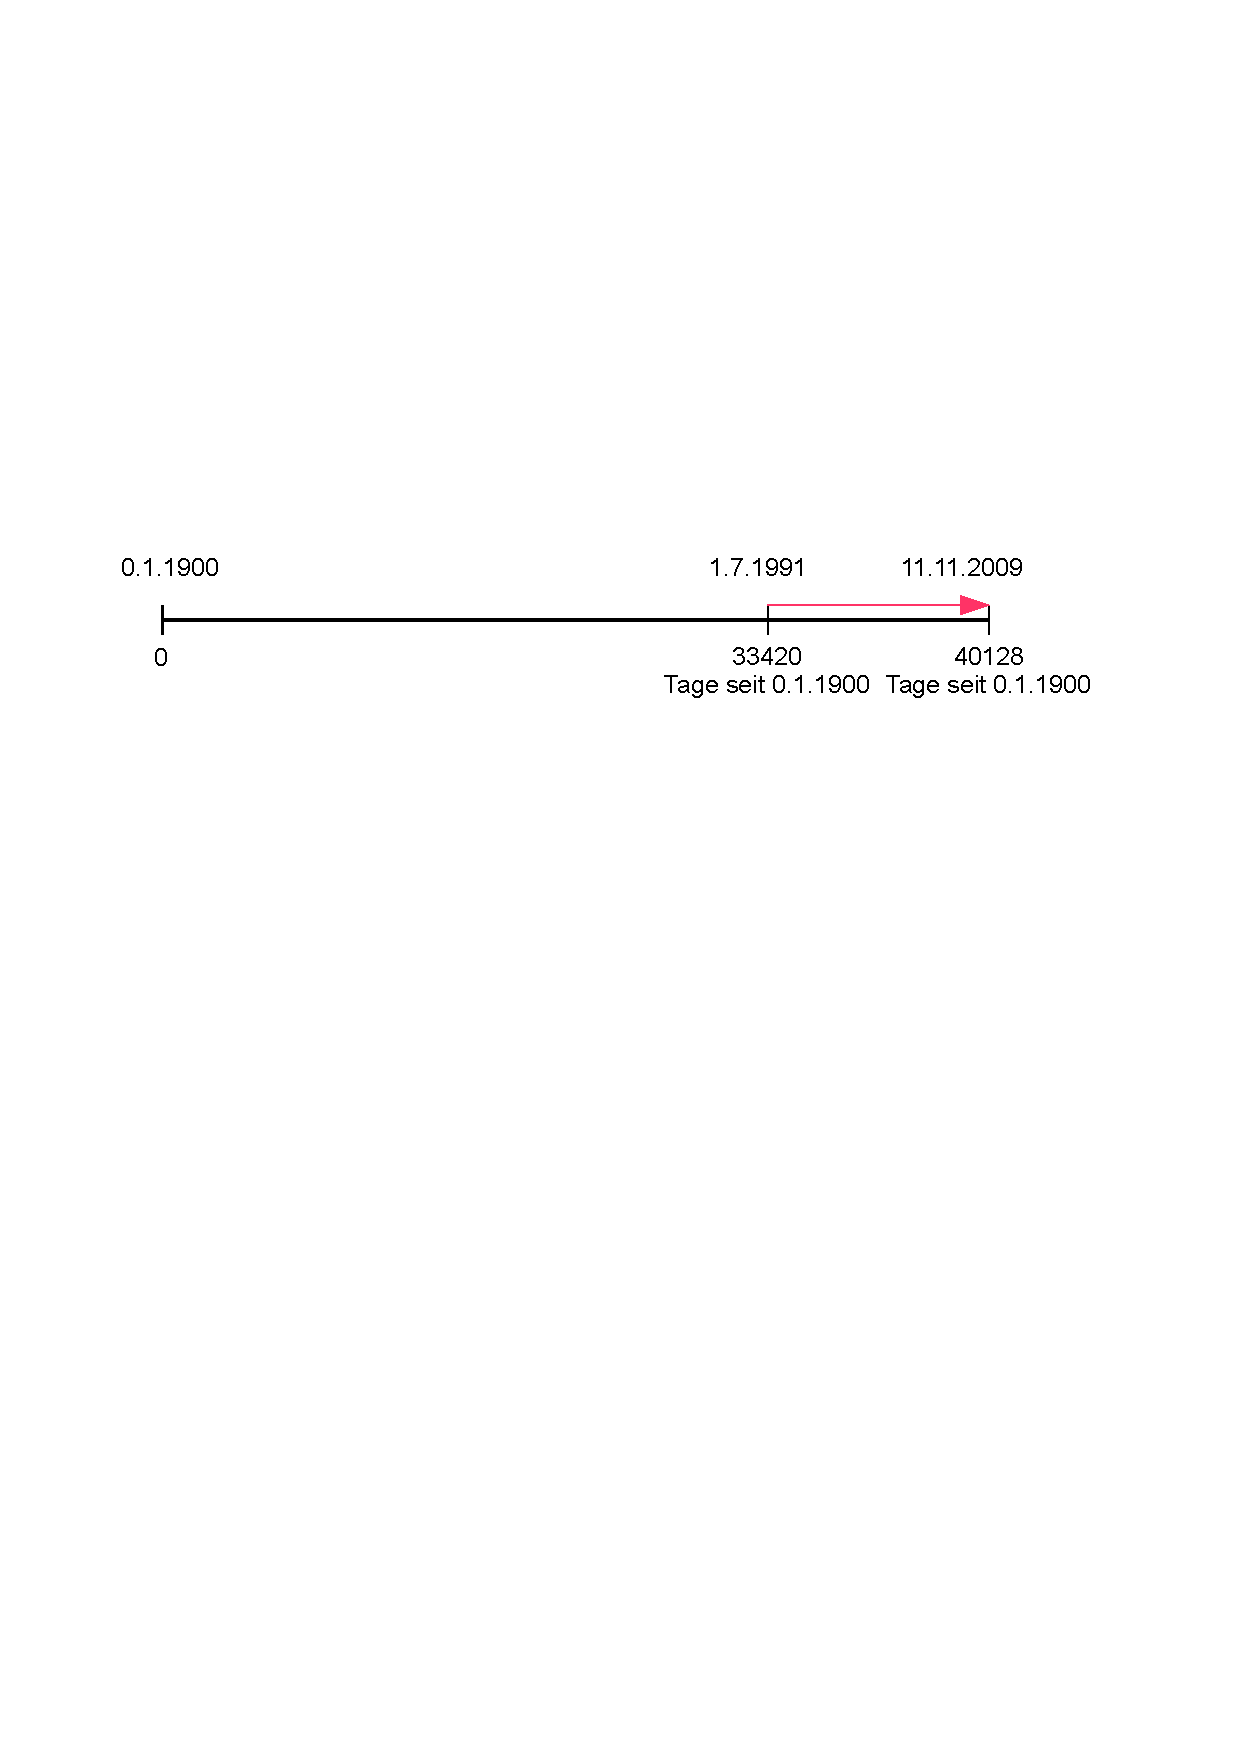
\includegraphics{_OpenOffice/datum2.pdf}
		\caption{Altersdifferenz auf der Zeitachse}
		\label{fig:datum2}

	\end{figure}


Aus der \figref{fig:datum2} kann man erkennen, dass zwischen dem 11.11.2009 und dem 1.7.1991 genau 40128-33420 Tage liegen, was 6708 Tagen entspricht. Tragen wir nun einmal diese einfache Formel ein und sehen uns das Ergebnis an.
%\placefigure[middle,force][fig:alter2]{}{\externalfigure[alter2]}
	\begin{figure}[H]
		\centering
		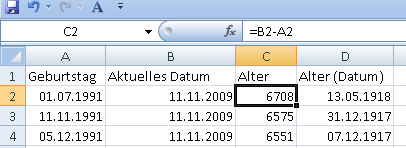
\includegraphics{images/alter2.png}
		\caption{Berechnete Altersdifferenzen}
		\label{fig:alter2}
	\end{figure}


In Zelle \xlc{C2} steht die Formel \stmt{=B29-A2}. In der Spalte \xlc{C9} ist das Alter in Tagen als Zahl formatiert zu sehen. In der Spalte \xlc{D} dagegen ist der Inhalt der Spalte \xlc{C} als Datum formatiert zu sehen. Es ist erkennbar, dass das Jahr 1917, beziehungsweise
1918, etwas mit dem Alter zu tun haben muss. In der unteren Abbildung ist die Erklärung dafür. Nehem Sie die Differenz der beiden Zeitpunkte und betrachten Sie diese vom Anbeginn der Microsoftschen Zeitrechnung aus.
%\placefigure[middle,force][fig:datum3]{}{\externalfigure[datum3]}
	\begin{figure}[H]
		\centering
		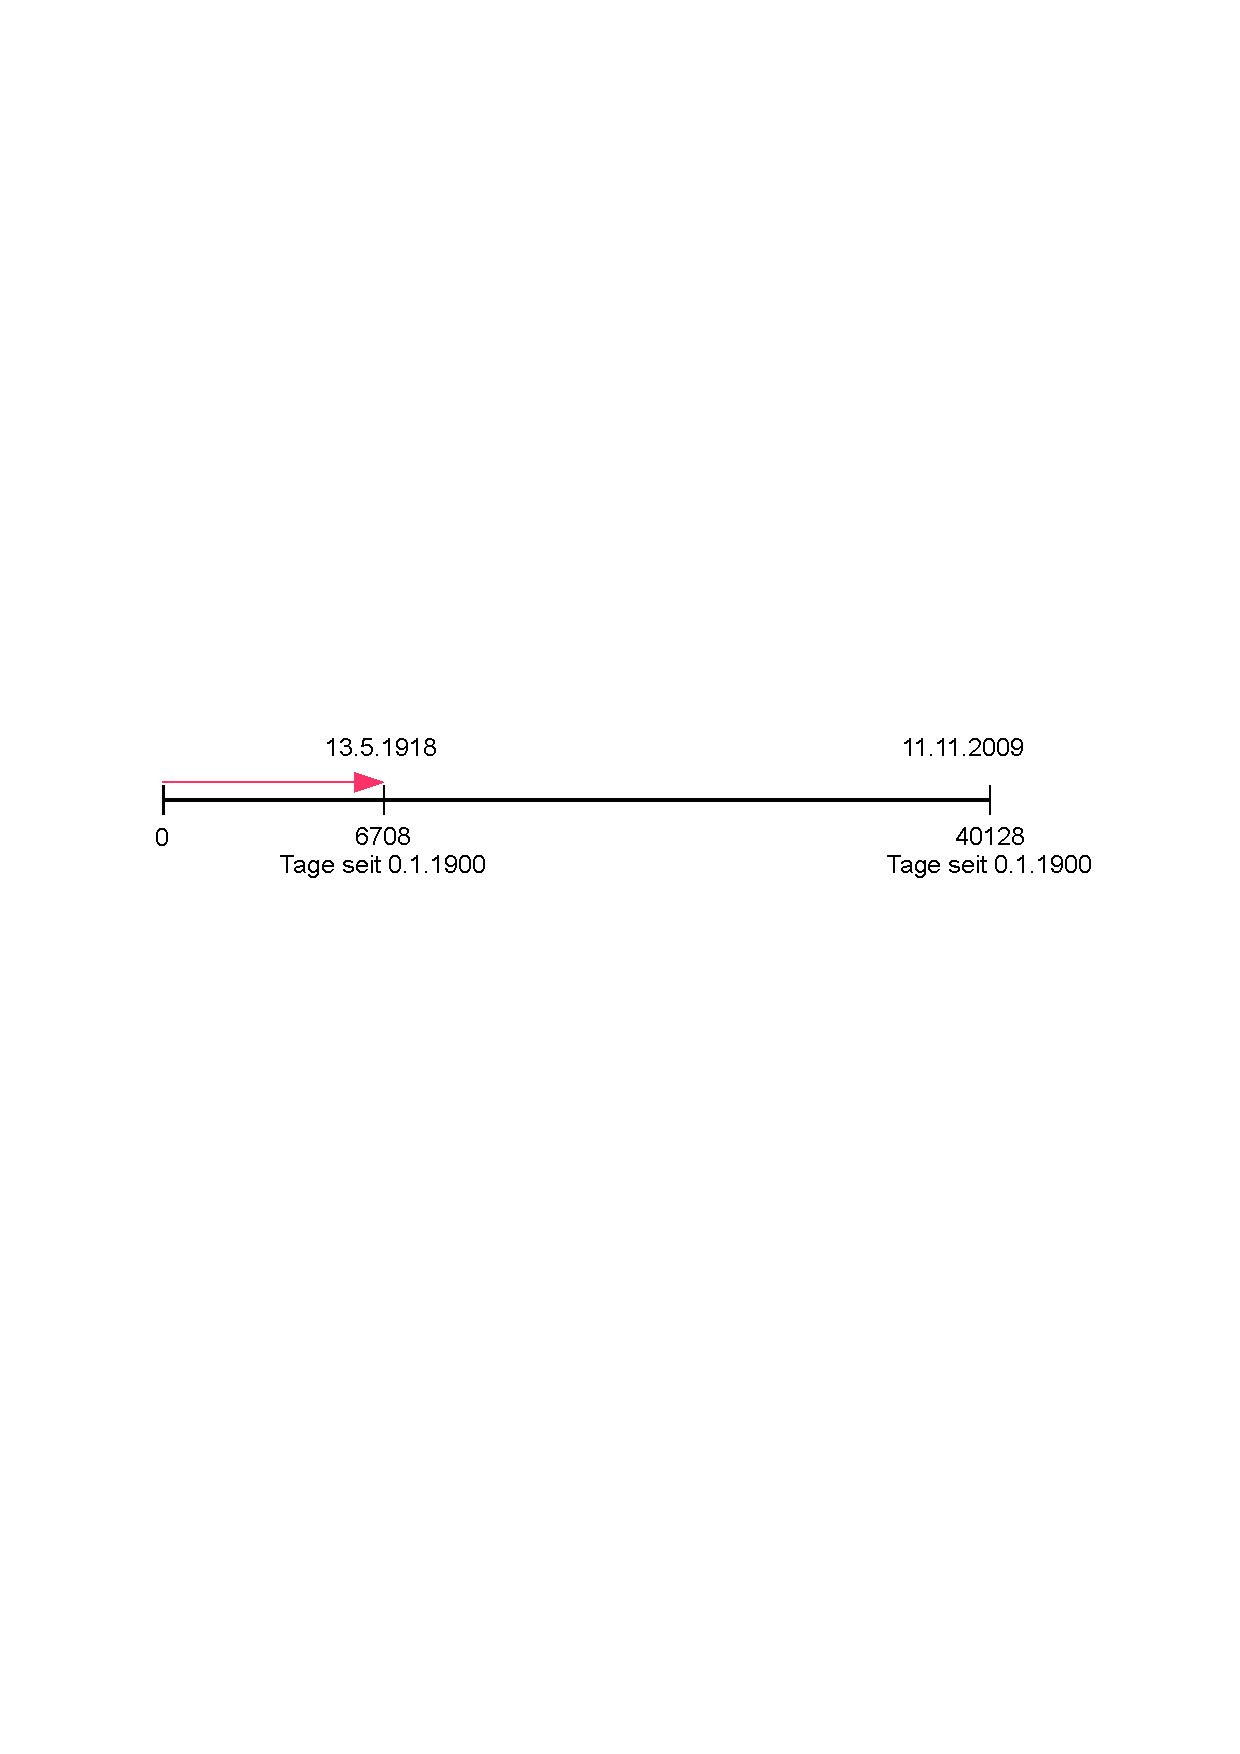
\includegraphics{_OpenOffice/datum3.pdf}
		\caption{Differenzalter auf der Zeitachse}
		\label{fig:datum3}
	\end{figure}



Um das eigentliche Alter in Jahre zu erhalten sind jetzt noch 2 Schritte notwendig
\begin{itemize}
	\smallitemize
	\item Mittels der Funktion \stmt{JAHR()} aus dem Differenzdatum nur die Jahreszahl extrahieren.\\
	Mit \stmt{=JAHR(B2-A2)} erhalten Sie 1917, beziehungsweise 1918
	\item Den Beginn der Microsoftschen Zeitrechnung, also 1900, abziehen
	Mit \stmt{=JAHR(B2-A2)-1900} erhalten Sie 17, beziehungsweise 18
\end{itemize}

Damit scheint das Ergebnis erreicht zu sein. Leider nur scheinbar, denn am Tag des Geburtstages wird ein falsches Alter angezeigt. Um das zu korrigieren, addiert man einfach einen Tag zur Differenz zwischen beiden Daten. Das Ergebnis sieht dann wie folgt aus.
%\placefigure[middle,force][fig:alter3]{}{\externalfigure[alter3]}
	\begin{figure}[H]
		\centering
		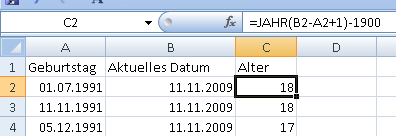
\includegraphics{images/alter3.png}
		\caption{Tatsächliche Altersdifferenz}
		\label{fig:alter4}
	\end{figure}

\subsection{Übersicht}

\begin{description}[labelindent=0cm, leftmargin=7cm, font=\mdseries, labelwidth=5cm,style=nextline]
	
	\item[\stmt{HEUTE()}] Liefert das aktuelle Datum\\
		Z.B.  \stmt{HEUTE()} $\Rightarrow$ 01.09.2015
	\item[\stmt{JETZT() }] Liefert das aktuelle Datum samt Uhrzeit\\ 
		Z.B. \stmt{JETZT} $\Rightarrow$ 21.02.2014 12:00:23
\item[\stmt{TAG(\syntax{Datum})}] Liefert den Tag eines Datums als Ganzzahl\\
		Z.B. \stmt{TAG(\upquote{21.02.2014})} $\Rightarrow$ 21
\item[\stmt{MONAT(\syntax{Datum})}] Liefert das Monat eines Datums als Ganzzahl\\
		Z.B. \stmt{MONAT("21.02.2014")} $\Rightarrow$ 2
\item[\stmt{JAHR(\syntax{Datum})}] Liefert das Jahr eines Datums als Ganzzahl\\
		Z.B: \stmt{JAHR("21.02.2014")} $\Rightarrow$ 2014
\item[\stmt{DATUM(\syntax{Jahr}; \syntax{Monat}; \syntax{Tag})}] Erstellt aus 3 Ganzzahlen ein Datum\\
	Z.B. Datum(21; 2; 2014) $\Rightarrow$ 41691\\
	Diese Funktion ist eine der wichtigsten Datumsfunktionen, weil Sie eine beliebige Addition oder Subtraktion von Jahren, Monaten und Tagen ermöglicht und daraus ein neues Datum erstellen kann.
\item[\stmt{MONATSENDE(\syntax{Datum}, \syntax{Monat})}] Liefert das Monatsende als Datum (Zahl) zurück, das eine bestimmte Anzahl von Monaten vor bzw. nach einem Datum liegt.\\
	Z.B. \stmt{("21.02.2014"; 3)} $\Rightarrow$ 31.05.2014
\item[\stmt{WOCHENTAG(\syntax{Datum}; \syntax{Typ})}] Liefert den Wochentag eines Datums als Ganzzahl zurück, wobei die Typangabe (Default = 1) entscheidet, welcher Wochentag mit welcher Zahl beginnt. (bei Default gilt 1=So, 2=Mo,3=Di,..)\\
Z.B. (z.B. \stmt{("21.02.2014"; 1)} $\Rightarrow$ 6
\item[\stmt{TEXT(\syntax{Datum};"\syntax{Format}") }] Gibt ein Datum entsprechend dem ausgewählten Format an\footnote{\url{https://support.office.com/de-at/article/TEXT-Funktion-20d5ac4d-7b94-49fd-bb38-93d29371225c?ui=de-DE&rs=de-AT&ad=AT}}.\\
	Z.B.  \stmt{TEXT("21.02.2014"; "TTT")} $\Rightarrow$ Fr
\item[\stmt{DATEDIF(\syntax{Startdatum}; \syntax{Enddatum}; \syntax{Einheit})}] Liefert die Differenz als Ganzzahl zwischen zwei Datumswerten. Als Einheit kann man "Y", "M" oder "D" angeben. Es ist zu beachten, dass das Startdatum immer vor dem Enddatum liegen muss.\\
Z.B. \stmt{DATEDIF(HEUTE(); "24.12.2014"; "D")} $\Rightarrow$ 306
\item[\stmt{ARBEITSTAG(\syntax{Startdatum};\syntax{Tage}; \syntax{Freitage}) }] Liefert das Datum des nächsten (oder zurückliegenden) Arbeitstages durch Addition oder Subtraktion von Tagen zu einem Startdatum unter Berücksichtigung eventueller Freitage (Matrix).
\item[\stmt{NETTOARBEITSTAGE(\syntax{Beginndatum}; \syntax{Enddatum}; \syntax{Freitage}) }] Liefert die Anzahl der Arbeitstage zwischen einem Anfangsdatum  und einem Enddatum unter Berücksichtigung eventueller Freitage (Matrix).
\item[\stmt{EDATUM(\syntax{Ausgangsdatum} ;\syntax{Monate})}] Liefert das Datum (Zahl) zurück, das eine bestimmte Anzahl von Monaten vor bzw. nach einem Ausgangsdatum liegt.\\
Z.B. \stmt{EDATUM("29.02.2016"; -12)} $\Rightarrow$ 28.02.2015
\item[\stmt{KALENDERWOCHE(\syntax{Datum}; \syntax{Typ}) }] Liefert die Kalenderwoche eines Datums als Ganzzahl zurück.\\
Typ 1: Woche mit dem 1.1. ist die 1. Kalenderwoche (amerikanisches System)\\
Typ 21: Woche, die den 1. Donnerstag im Jahr hat, ist die Kalenderwoche 1 oder die den 4.1. beinhaltet (entspricht ISO EU-Standard).
\end{description}



\subsection{Zusammenfassung}
\begin{itemize}
	\item In Excel werden Datumswerte als Ganzzahl interpretiert. Das Standard-Datumsystem basiert darauf, dass der 1.1.1900 der Zahl 1 entspricht. Das letzte interpretierbare Datum ist der 31.12.9999, was der Zahl 2.958.465 entspricht.
	\item Auf Grund des Jahrtausendwechsels sind Jahreszahlen im vierstelligen Format anzugeben. Die zweistelligen Jahreszahlen 00-29 werden als 2000 bis 2029 interpretiert, 30 bis 99 hingegen als 1930 bis 1999.

	\item Da In Excel Datums- und Uhrzeitangaben als Zahlen repäsentiert werden, kann man daher auch mittels mathemathischer Operatoren, wie Addition und Subtraktion, mit Datumswerten rechnen.	
	
\end{itemize}


\section{Uhrzeitfunktionen}

\subsection{Allgemeines}

Für die Uhrzeit, oder generell Zeitdarstellung, wird einfach der Nachkommateil des Datums herangezogen. 0,5 entspricht hier genau 12 Uhr, 0,75 wäre 18 Uhr. Fügt man nun Datum und Uhrzeit zusammen, so erhält man mit 40128,5 den 11.11.2009 und 12 Uhr Mittags.

Eine Funktion, welche für Zeitberechnungen immer wieder verwendet wird, ist \xlf{Zeit}, mit der man getrennte Stunden, Minuten und Sekunden zu einem Zeitwert zusammenführt.



\subsection{Übersicht}
\begin{description}[labelindent=0cm, leftmargin=7cm, font=\mdseries, labelwidth=5cm,style=nextline]
\item[\stmt{STUNDE(\syntax{Uhrzeit})}] Liefert die Stunde einer Uhrzeit als Ganzzahl\\
Z.B. \stmt{STUNDE("12:34:23")} $\Rightarrow$ 12
\item[\stmt{MINUTE(\syntax{Uhrzeit})}] Liefert die Minute einer Uhrzeit als Ganzzahl\\
Z.B. \stmt{MINUTE("12:34:23)"} $\Rightarrow$ 34
\item[\stmt{SEKUNDE(\syntax{Uhrzeit})}] Liefert die Sekunde einer Uhrzeit als Ganzzahl\\
Z.B. \stmt{SEKUNDE("12:34:23")} $\Rightarrow$ 23
\item[\stmt{ZEIT(\syntax{Stunde}; \syntax{Minute}; \syntax{Sekunde}) }] Erstellt aus drei Ganzzahlen eine Uhrzeit\\
Z.B. \stmt{ZEIT(12; 34; 23)} $\Rightarrow$ 12:34:23 \\$\Rightarrow$ 0,523877314814815
\end{description}


% http://tex.stackexchange.com/questions/58757/how-do-you-put-a-character-in-the-margin-using-an-environment


\begin{infobox}%
Die \stmt{ZEIT()} Funktion eignet sich wie die \stmt{DATUM()}Funktion, um aus Addition oder Subtraktion von Stunden, Minuten und Sekunden eine neue Uhrzeit zu bekommen. Es ist allerdings zu beachten, dass bei einem Überschreiten der 24 Stunden die Zeitfunktion allfällige Tage abschneidet. So ergibt \stmt{ZEIT(27; 0; 0)} nicht den Wert 1,125 sondern 0,125, was der Uhrzeit von 3 Uhr entspricht.
\end{infobox}


Wenn als Beispiel zu dem Zeitpunkt 15.03.2014 11:00:00 eine Zeit von 30 Stunden, 20 Minuten und 10 Sekunden addiert werden soll bringt die Formel
$$ =\text{\stmt{"15.3.2014 11:00:00" + ZEIT(30;20;10)}}$$
das nicht richtige  Ergebnis: 15.3.2014 17:20:10!
\begin{lightbulbbox}
Um dieses Problem zu lösen, ist es ratsam, prinzipiell für Zeitoperationen Stunden, Minuten und Sekunden in Bruchteile eines Tages umzurechnen. Also lautet die Formel für die korrekte Berechnung
$$ =\text{\stmt{"15.03.2014 11:00:00" + 30/24 + 20/24/60+10/24/60/60}}$$
welche das korrekte Ergebnis 16.03.2014 17:20:10 liefert.
\end{lightbulbbox}



\subsection{Zusammenfassung}

	
\begin{itemize}
	\item  Uhrzeiten werden als Bruchteil von 1 angesehen. So entspricht die Zahl 0,5 der Uhrzeit 12:00 oder 0,375 entspricht 09:00. Der Termin 05.03.2014 11:15 entspricht daher dem Zahlenwert 41703,46875.

	\item Da In Excel Datums- und Uhrzeitangaben als Zahlen repäsentiert werden, kann man daher auch mittels mathemathischer Operatoren, wie Addition und Subtraktion, mit Datumswerten rechnen.	
	
\end{itemize}
\pagebreak
\section{\stmt{WENN} Funktion}

$$ \text{\stmt{WENN(\syntax{Bedingung}; [\syntax{Dann\_Wert}]; [\syntax{Ansonsten\_Wert}])}}$$

	\begin{figure}[H]
		\centering
			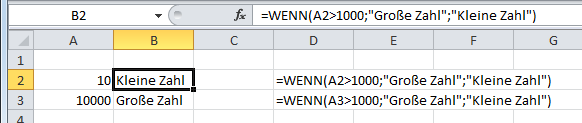
\includegraphics[scale=0.7]{images/wenn_1b}
			\caption{\stmt{WENN} Funktion}
		\label{fig:wenn}
	\end{figure}


Die \stmt{WENN} Funktion liefert in einfachster Form einen Wert zurück. Wenn die \syntax{Bedingung} als WAHR ausgewertet wird, liefert sie den \syntax{Dann\_Wert}, wird sie als FALSCH ausgewertet liefert sie den \syntax{Ansonsten\_Wert}.


Jede \stmt{WENN} Funktion, auch eine verschachtelte, wird automatisch beendet, wenn ein Zweig durchlaufen wird. \stmt{WENN} Funktionen können bis zu 64-fach ineinander verschachtelt werden. Achten Sie bei verschachtelten \stmt{WENN} Funktionen, dass Ihre numerischen Abgrenzungen in den Bedingungen einer logischen Abfolge gleichen.

Im untenstehenden Beispiel ist eine verschachtelte \stmt{WENN} Funktion dargestellt. Ist das Alter mindestens 65 Jahre, dann wird "`ALT"' angezeicht, ist es das nicht, wird danach geprüft, ob das Alter zumindest 35 Jahre ist. Ist das zutreffend, wird "`MITTEL"' angezeigt. Ist die Person unter 35 Jahren, dann wird "`JUNG"' ausgegeben.

	\begin{figure}[H]
		\centering
			%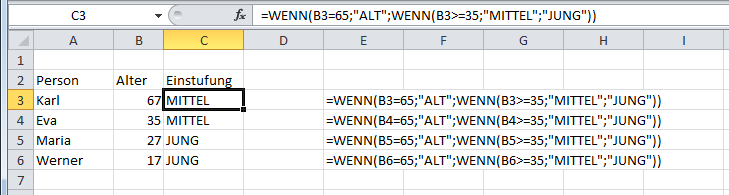
\includegraphics[width=16cm]{images/wenn_verschachtelt_b}
			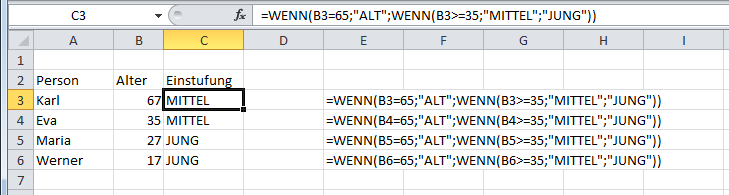
\includegraphics[scale=0.7]{images/wenn_verschachtelt_b}
		\caption{Verschachtelte \stmt{WENN} Funktion}
		\label{fig:wenn_verschachtelt}
	\end{figure}

\begin{lightbulbbox}
Grundsätzlich gilt die Merkregel:\\
Numerische Grenzen von großem nach kleinem Wert immer mit $>$ oder $>=$\\
Numerische Grenzen von kleinem nach großem Wert immer mit $<$ oder$<=$
\end{lightbulbbox}

\section{\stmt{UND}  Funktion}

$$ \text{\stmt{UND( \syntax{Bedingung\_1}; \syntax{Bedingung\_2}; \ldots; \syntax{Bedingung\_255})}} $$

Die \stmt{UND} Funktion gibt WAHR zurück, wenn alle Bedingungen WAHR sind.

\begin{description}[labelindent=0cm, leftmargin=3cm, font=\mdseries, labelwidth=3cm,style=nextline]
\item[Beispiele] \stmt{=UND( 1>2 ; 2<3 )} $\Rightarrow$ FALSCH\\
\stmt{=UND( 1>0 ; 8/4=2 )} $\Rightarrow$ WAHR
\end{description}
%
Die \stmt{UND} Funktion kommt sehr häufig in Formeln mit einer \stmt{WENN} Bedingung vor.
%
	\begin{figure}[H]
		\centering
			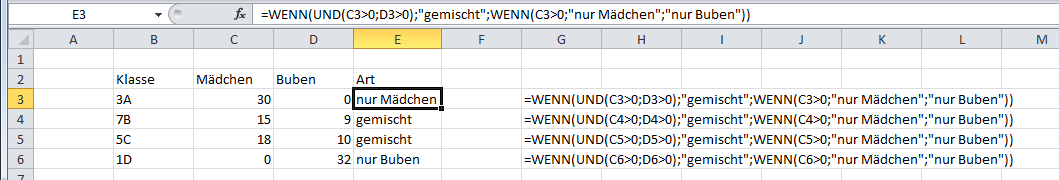
\includegraphics[width=16cm]{images/und_mit_wenn_b}
%			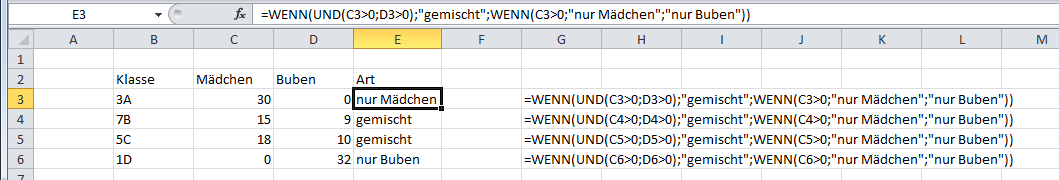
\includegraphics[scale=0.7]{images/und_mit_wenn_b}
		\caption{\stmt{WENN} und \stmt{UND} in einer Formel}
		\label{fig:wenn_mit_und}
	\end{figure}


\section{\stmt{ODER} Funktion}

$$ \text{\stmt{ODER( \syntax{Bedingung\_1}; \syntax{Bedingung\_2}; \ldots; \syntax{Bedingung\_255})}} $$

Die \stmt{ODER} Funktion gibt WAHR zurück wenn zumindest eine der Bedingungen WAHR ergibt.

\begin{description}[labelindent=0cm, leftmargin=3cm, font=\mdseries, labelwidth=3cm,style=nextline]
\item[Beispiele] \stmt{=ODER( 1<0 ; 8/4=2 )} $\Rightarrow$ WAHR \\
\stmt{=ODER( 1=2 ; 4/0,5=2 )} $\Rightarrow$ FALSCH
\end{description}
%
%
	\begin{figure}[H]
		\centering
%			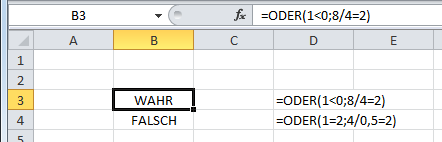
\includegraphics[width=11cm]{images/oder_1b}
			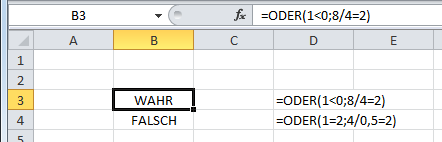
\includegraphics[scale=0.7]{images/oder_1b}
		\caption{\stmt{ODER} in einer Formel}
		\label{fig:oder}
	\end{figure}


\section{Matrixfunktionen}

Matrixfunktionen bieten uns die Möglichkeit, nach bestimmten Kriterien Werte aus Listen oder Bereichen zu entnehmen, ihre Positionen zu bestimmen oder bieten uns Hilfestellungen dafür an. 


\subsection{\stmt{VERGLEICH}}

$$ \text{\stmt{   VERGLEICH(\syntax{Suchkriterium}; \syntax{Suchmatrix}; [\syntax{Vergleichstyp}])  }}$$

Die \stmt{VERGLEICH} Funktion wird dann verwendet, wenn man nicht den Wert aus einer Spalte oder Zeile haben will, sondern die Position bezogen auf die Suchmatrix.


\begin{description}[labelindent=0cm, leftmargin=3cm, font=\mdseries, labelwidth=3cm,style=nextline]
\item[\syntax{Suchkriterium}] Wert nach dem in der \syntax{Suchmatrix} gesucht werden soll
\item[\syntax{Suchmatrix}] ist entweder ein Zeilenbereich, z.B. \stmt{\upquote{A2:H2}}, oder ein Spaltenbereich, z.B. \stmt{\upquote{A2:A6}}, in dem gesucht werden soll.
\item[\syntax{Vergleichstyp}] %
	\begin{description}[labelindent=0cm, leftmargin=2cm, font=\mdseries, labelwidth=2cm,style=nextline]
	\item[1 (default)] Sucht nach dem größtem Wert, der kleiner oder gleich dem Suchkriterium ist. Die Suchmatrix muss daher zwingend \textsl{aufsteigend} sortiert sein.
	\item[0] Sucht exakt das Suchkriterium in der Suchmatrix. Das Suchkriterium muss in
der Suchmatrix vorkommen, die Suchmatrix muss aber nicht sortiert sein.
	\item[-1] Sucht nach dem kleinsten Wert, der größer oder gleich dem Suchkriterium ist.
Die Suchmatrix muss daher zwingend \textsl{absteigend} sortiert sein.
	\end{description}

\end{description}

Im folgenden Beispiel ist das Suchkriterium der Wert 245. \stmt{VERGLEICH} sucht nun im angegebenen Suchbereich jene Zeile, in der der gesuchte Wert größer gleich dem Wert in der Zeile, aber kleiner als der Wert in der nächsten Zeile ist. In diesem Falle, ist es hier die Zeile mit dem Wert 200. Der ist ja kleiner als unser gesuchter Wert. Und der Wert in der nächsten Zeile ist schon größer als unser gesuchter Wert. Der gesuchte Wert ist also in der zweiten Zeile des Suchbereiches und daher liefert die Formel den Wert 2.

	\begin{figure}[H]
		\centering
%			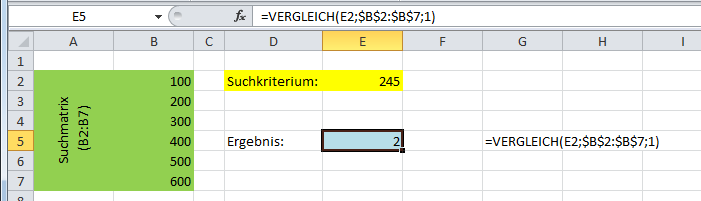
\includegraphics[width=16cm]{images/vergleich_1b}
			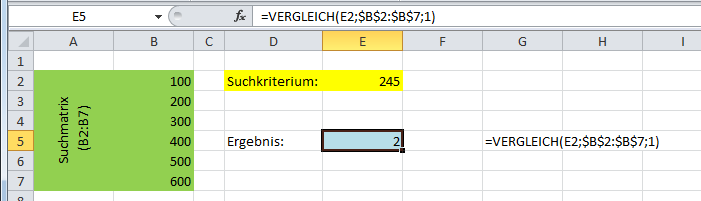
\includegraphics[scale=0.7]{images/vergleich_1b}
		\caption{\stmt{VERGLEICH} in einem Beispiel}
		\label{fig:vergleich_1}
	\end{figure}
	
	
\begin{infobox}%
Wenn der Suchwert kleiner als der kleinste Wert in der Suchmatrix ist, dann wird ein Fehler \stmt{\#NV} retourniert. Fehler wie \stmt{\#NV}, \stmt{\#Wert!}, \stmt{\#Bezug!}, \stmt{\#Div/0!}, \stmt{\#Num!}, \stmt{\#Name!} oder \stmt{\#Null!} können mit der Funktion \stmt{WENNFEHLER(\syntax{Wert}; \syntax{Wert falls Fehler})} abgefangen werden.
\end{infobox}

	\begin{figure}[H]
		\centering
%			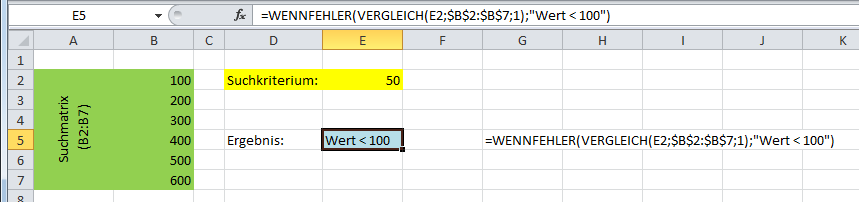
\includegraphics[width=16cm]{images/vergleich_2b}
			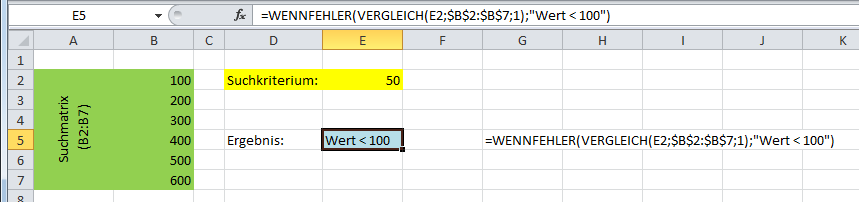
\includegraphics[scale=0.7]{images/vergleich_2b}
		\caption{\stmt{VERGLEICH} mit fehlerhaftem Wert}
		\label{fig:vergleich_fehler}
	\end{figure}

\subsection{\stmt{INDEX} (Matrixversion)}

$$ \text{ \stmt{INDEX( \syntax{Matrix}; \syntax{Zeile}; \syntax{Spalte})}}$$

Die \stmt{INDEX} Funktion liefert aus einer Matrix genau jenen Wert, der im angegebenen Schnittpunkt einer Zeile und einer Spalte steht. Besteht die Matrix aus nur einem Zeilenbereich oder einem Spaltenbereich kann das Argument der Zeile bzw. Spalte weggelassen werden. 
%
Im einfachsten Anwendungsfall, der sehr selten vorkommt, weiß man, in welcher Zeile der Matrix der gewünschte Spaltenwert zu suchen ist. In der \figref{fig:matrix}  wird der Preis der Zitrone gewünscht, welche in der dritten Zeile der Matrix steht.
	\begin{figure}[H]
		\centering
%			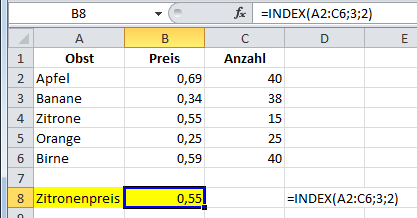
\includegraphics[width=8cm]{images/matrix_1b}
			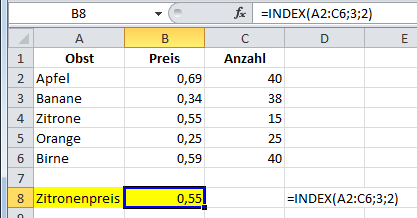
\includegraphics[scale=0.7]{images/matrix_1b}
		\caption{\stmt{MATRIX} Funktion}
		\label{fig:matrix}
	\end{figure}
%
Normalerweise kennt man entweder die Spalte nicht, die Zeile nicht oder auch beides gemeinsam nicht. Wenn das obige Beispiel derart erweitert wird, dass auch die Obstsorte wählbar ist, dann würde die Formel folgendermaßen aussehen.
%
	\begin{figure}[H]
		\centering
%			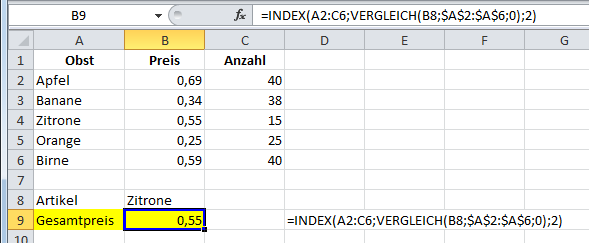
\includegraphics[width=12cm]{images/matrix_mit_vergleich_b}
			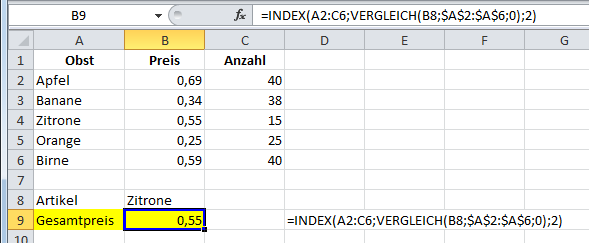
\includegraphics[scale=0.7]{images/matrix_mit_vergleich_b}
		\caption{\stmt{MATRIX} Funktion mit \stmt{VERGLEICH}}
		\label{fig:matrix_mit_vergleich}
	\end{figure}
%
\begin{infobox}%
Es ist wichtig, dass man eventuelle Spalten- oder Zeilenbeschriftungen \textit{nicht} zum Matrixbereich hinzuzählt. Der Matrixbereich ist nur der Wertebereich.
\end{infobox}

\subsection{\stmt{INDEX} (Bezugsversion)}

$$ \text{\stmt{INDEX( \syntax{Matrix}; \syntax{Zeile}; \syntax{Spalte}; [\syntax{Bereich}] )}}$$


Liefert den Bezug jener Zelle, auf die sich Zeile und Spalte in dem angegebenen Bezug (=Zellbereich) beziehen. Für den Paramater \syntax{Bezug} können auch mehrere, voneinander unabhängige Zellbereiche durch \stmt{()} eingeschlossen, angegeben werden.

\begin{description}[labelindent=0cm, leftmargin=3cm, font=\mdseries, labelwidth=3cm,style=nextline]
\item[Bereich]Falls mehrere Bezüge angegeben werden, bezieht sich die Bereichsnummer beginnend mit 1, dem Defaultwert, auf den jeweiligen Bezugsbereich.
\end{description}
%
	\begin{figure}[H]
		\centering
%			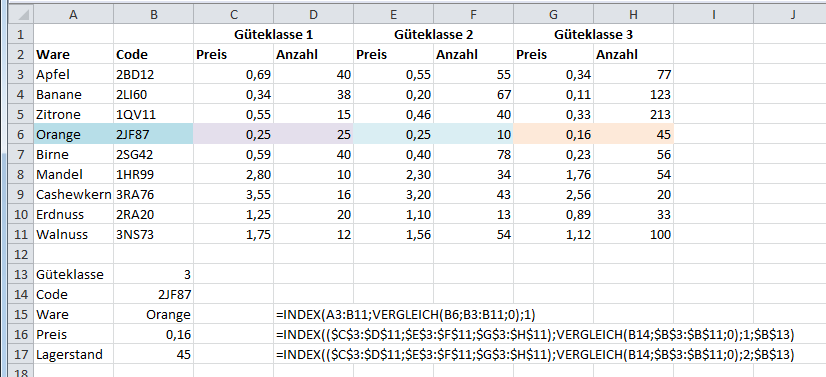
\includegraphics[width=16cm]{images/index_mit_bezug_b}
			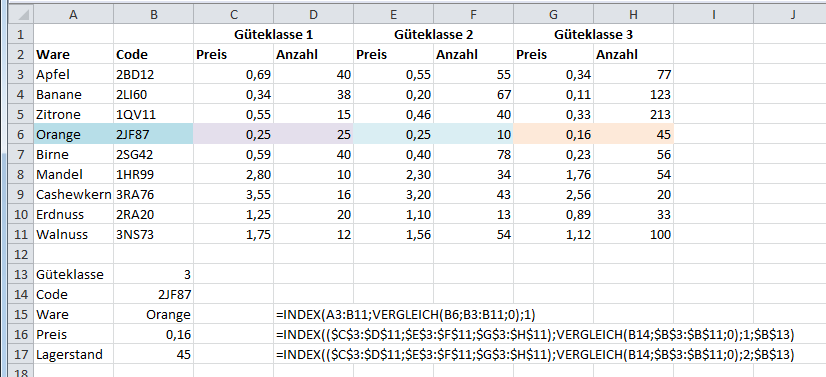
\includegraphics[scale=0.7]{images/index_mit_bezug_b}
		\caption{\stmt{INDEX} Funktion mit mehreren Bereichen}
		\label{fig:matrix_mit_bezug}
	\end{figure}
%
Schauen wir uns die Formel für den Lagerstand in Zelle \xlc{B17} näher an und teilen die einzelnen Parameter zur näheren Erklärung in ihre Einzelteile auf%
$$ \text{ \stmt{=INDEX((\$C\$3:\$D\$11;\$E\$3:\$F\$11;\$G\$3:\$H\$11);VERGLEICH(B14;\$B\$3:\$B\$11;0);2;\$B\$13)} }$$

\begin{description}[labelindent=0cm, leftmargin=8cm, font=\mdseries, labelwidth=8cm,style=nextline]
\item[\stmt{(\$C\$3:\$D\$11;\$E\$3:\$F\$11;\$G\$3:\$H\$11)}]Der erste Parameter umfasst die drei verschiedenen Bereiche mit Preis und Lagerstand.
\item[\stmt{VERGLEICH(B14;\$B\$3:\$B\$11;0)}] Danach wird über die \stmt{VERGLEICH} Funktion die Zeile ermittelt, welche den gewünschten Wert enthält. Ind diesem Fall wird nach dem Code, welcher in \stmt{B14} angegeben ist, im Bereich \stmt{\$B\$3:\$B\$11} gesucht. Und das auf genaue Übereinstimmung.
\item[\stmt{2}] Da der Lagerstand gewünscht ist, soll aus der Matrix der Wert der zweiten Spalte zurückgegeben werden.
\item[\stmt{\$B\$13}] Im letzten Parameter wird nun bestimmt, aus welchem der im ersten Parameter angegebenen Bereiche der Wert genommen wird. Im obigen Beispiel bezeichnet die 3 der Güteklasse auch den dritten Bereich
\end{description}
	
\begin{infobox}%
Es ist absolut wichtig, dass mehrere Bereiche immer durch Klammern \stmt{()} umgeben sind, da sonst ein Fehler ausgegeben wird.
\end{infobox}

\subsection{Beispiel zu \stmt{INDEX} und \stmt{VERGLEICH}}

Die beiden Excel Funktionen \stmt{INDEX} und \stmt{VERGLEICH} arbeiten sehr oft zusammen und daher werden sie hier gemeinsam anhand eines Beispieles eines Obsthändlers erklärt, der wissen will wieviele Melonen im März verkauft wurden.

%\placefigure[middle,force]{}{\externalfigure[indexxls]}
	\begin{figure}[H]
		\centering
%			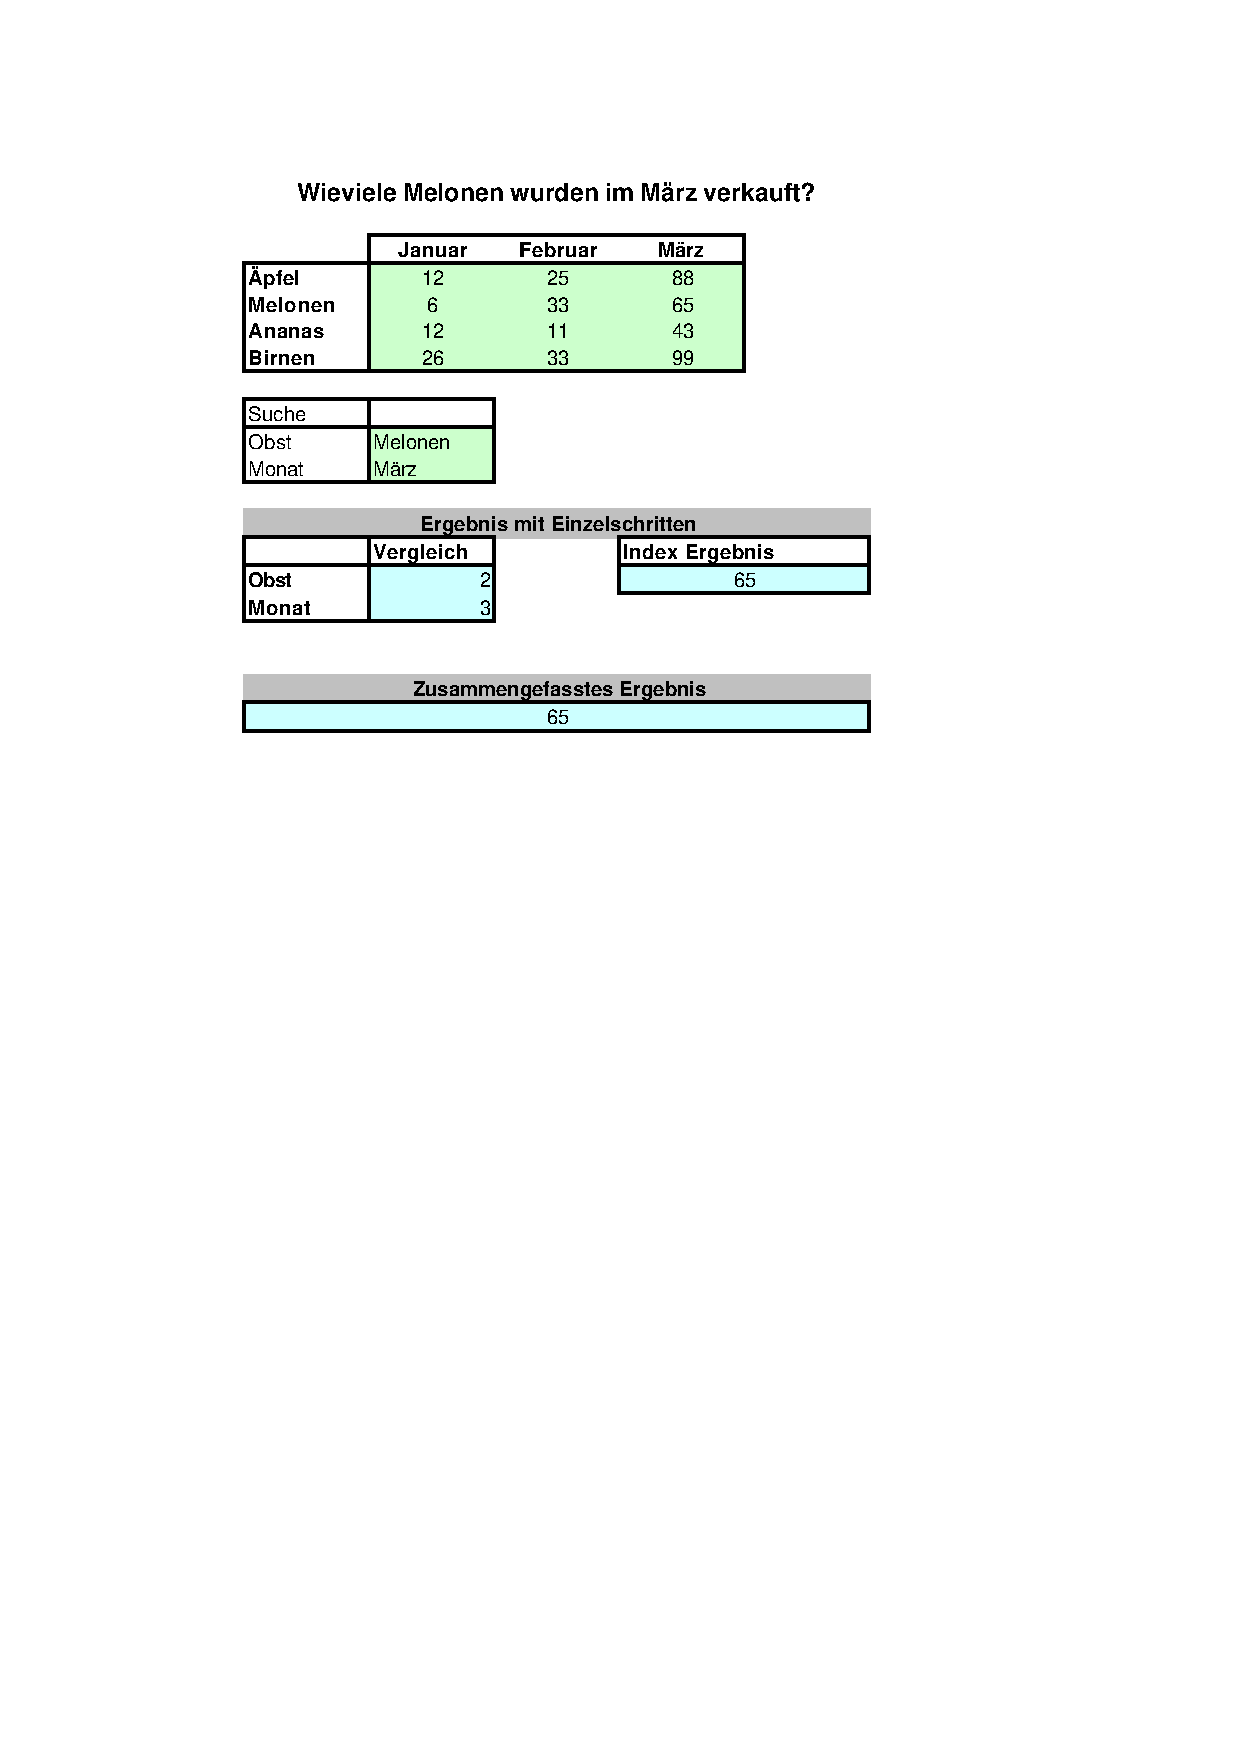
\includegraphics{images/Index_Grundbeispiel}
			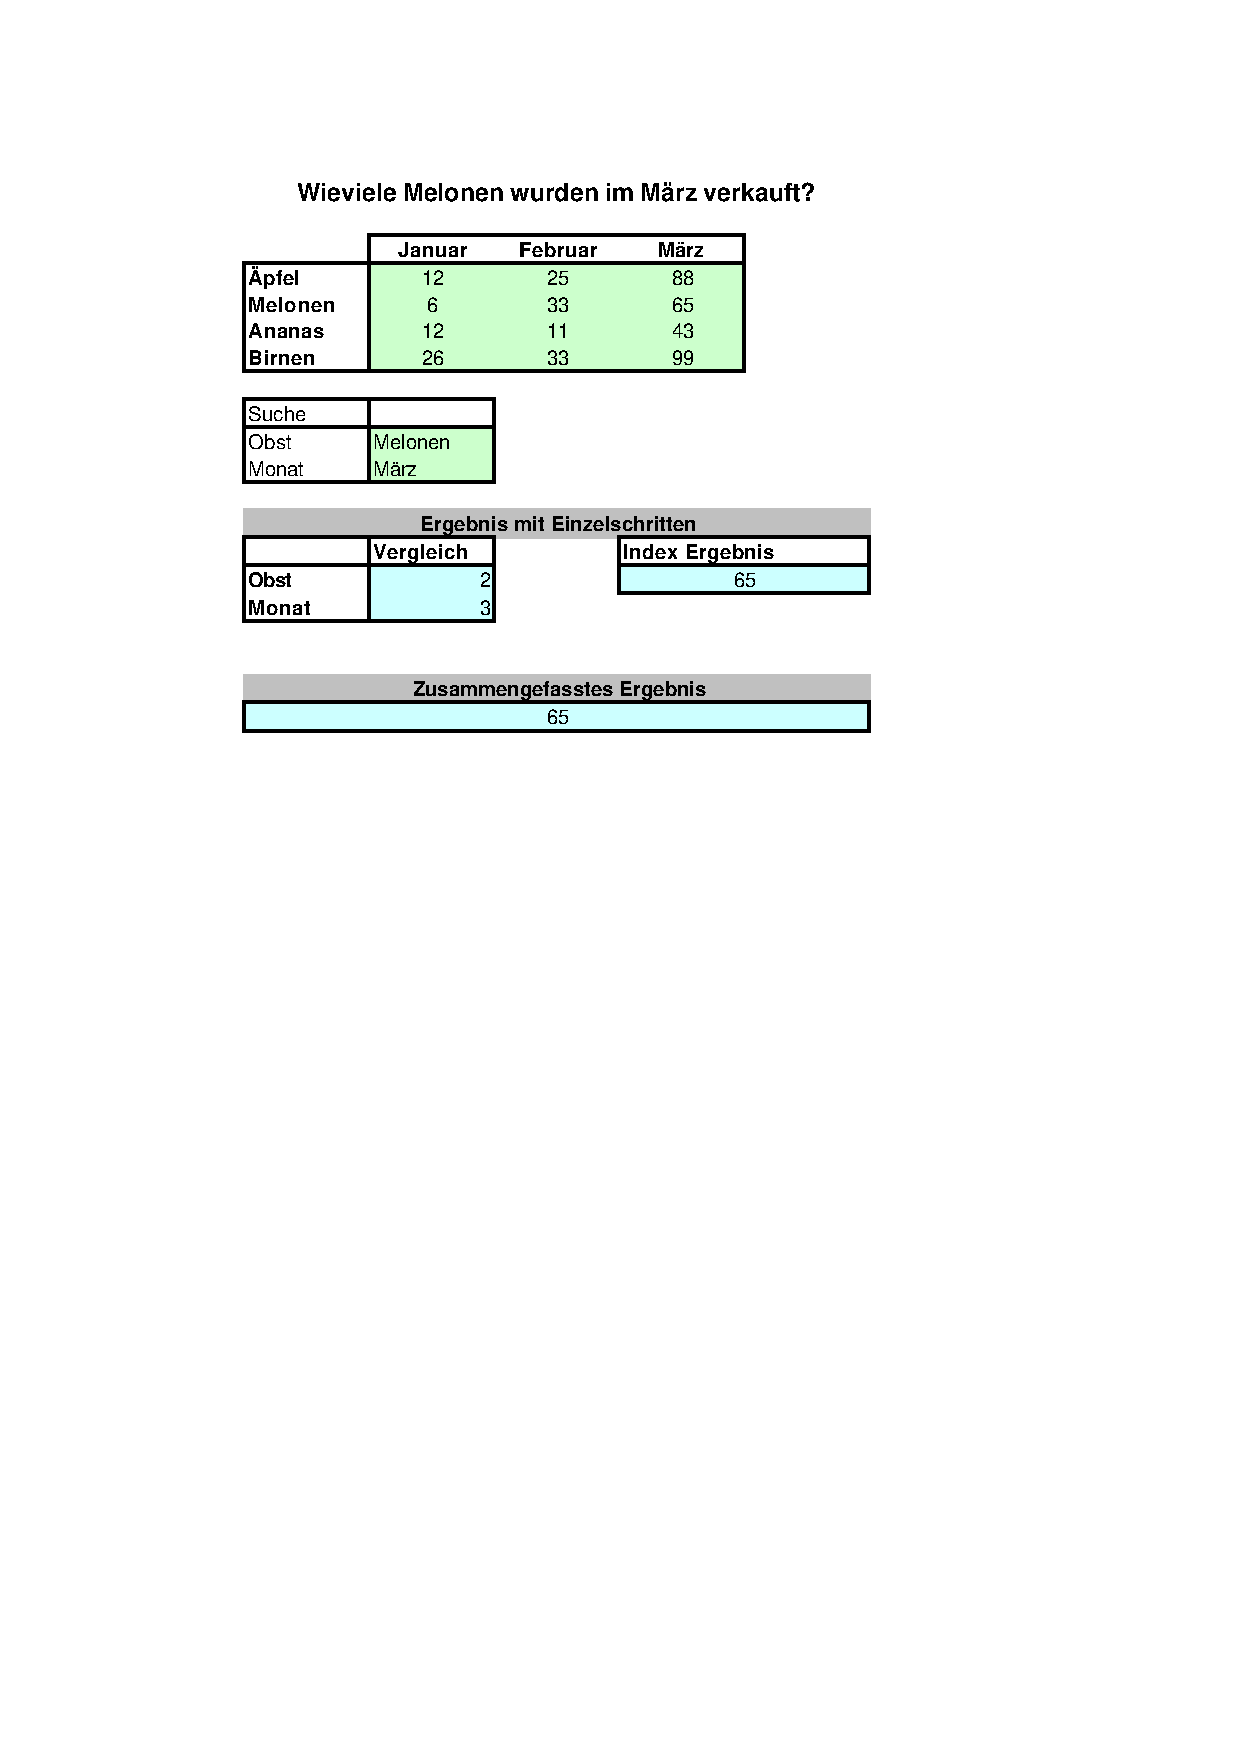
\includegraphics[scale=0.7]{images/Index_Grundbeispiel}
		\caption{Verkaufsliste des Obsthändlers}
		\label{fig:index_grundbeispiel}
	\end{figure}

Sieht man sich die Tabelle im Bereich \stmt{C5:E8} an, kann man erkennen, dass der gesuchte Wert der Schnittpunkt der Zeile 6, für die Melonen, und der Spalte E, für den Monat März, ist. Auf die Matrix bezogen ist der gesuchte Wert in der zweiten Zeile und der dritten Spalte. Die Spalten- und Reihenbezeichnung darf hier, wie bereits oben erwähnt, nicht miteinbezogen werden.


%\placefigure[middle,force]{}{\externalfigure[indexmatrix]}
	\begin{figure}[H]
		\centering
%			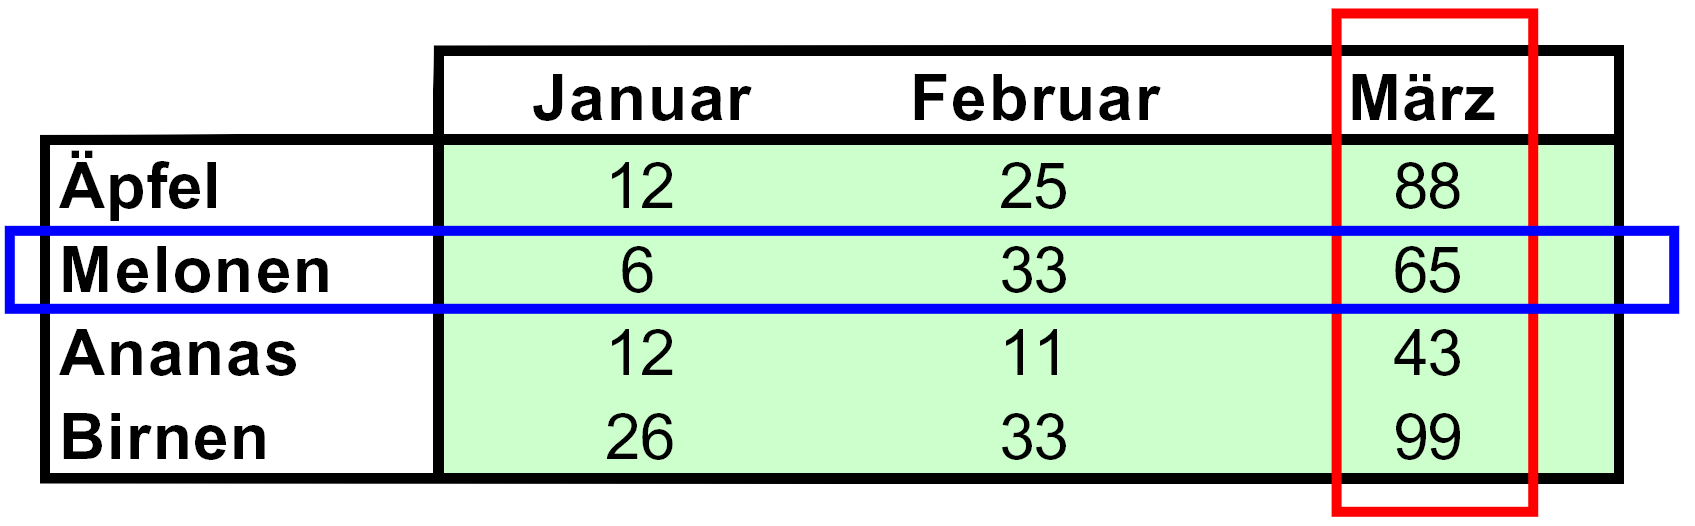
\includegraphics{images/index_matrix}
			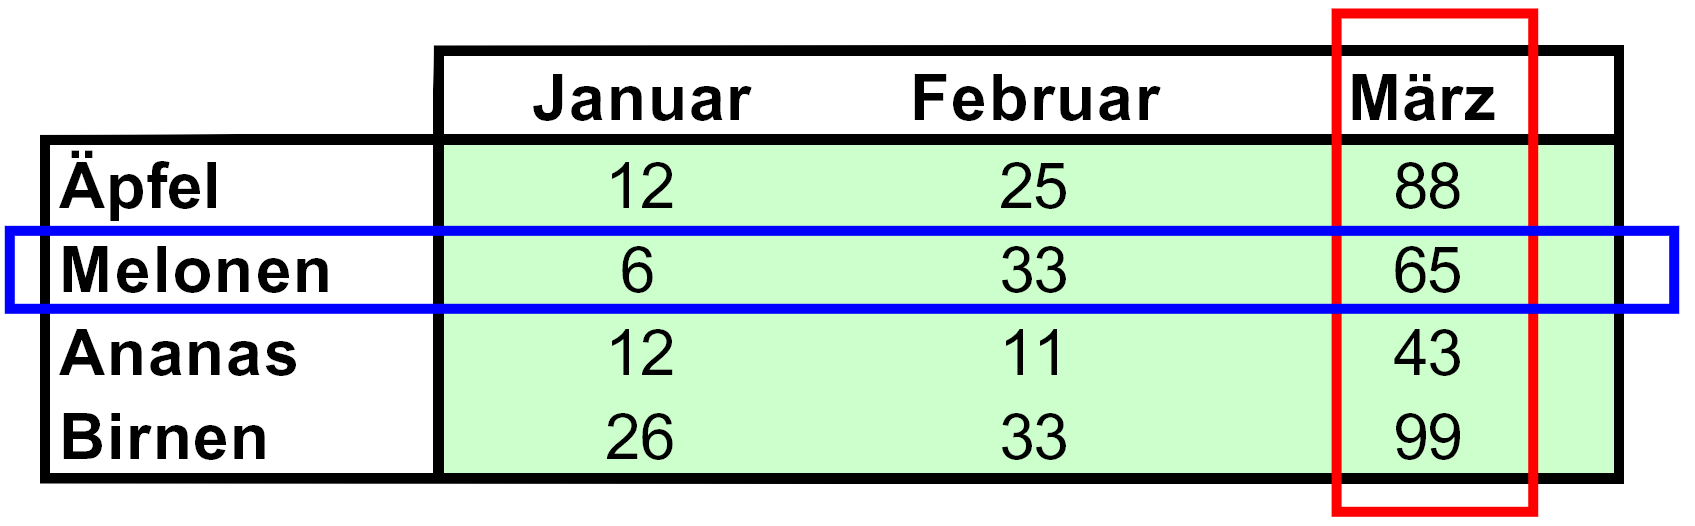
\includegraphics[scale=0.7]{images/index_matrix}
		\caption{Schnittpunkt mit dem gesuchten Wert}
		\label{fig:index_matrix}
	\end{figure}

Jetzt bleibt noch die Frage wie man die richtige Zeile und Spalte findet. Das einfachste ist, im Bereich \xlc{B5:B8} nach dem Wort Melonen und im Bereich \xlc{C4:E4} nach März zu suchen. Dafür wird die Excel Funktion \stmt{VERGLEICH} angewendet, welche in einem Suchbereich nach dem Suchkriterium gesucht. Man erhält die relative Position des gesuchten Elementes im Suchbereich.%
$$ \text{ \stmt{=VERGLEICH( \syntax{Suchkriterium}; \syntax{Suchbereich}; \syntax{Vergleichstyp})} }$$


\begin{figwindow}[0,r,{
		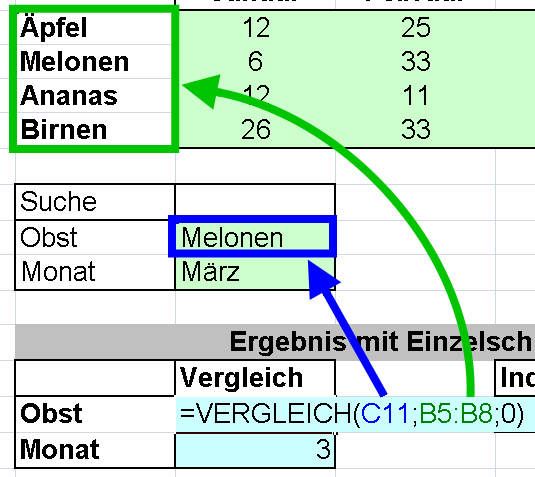
\includegraphics[width=5cm]{images/matrix_melonen}
%		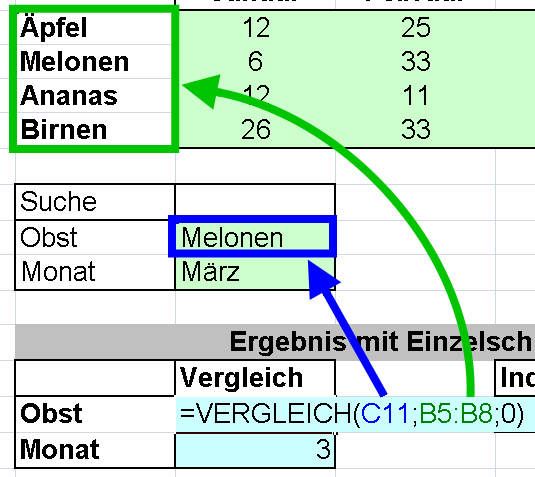
\includegraphics[scale=0.7]{images/matrix_melonen}
		\label{fig:matrixmelonen}} , {Melonen}
]
Zuerst wird in \xlc{C16} die Zeile der Matrix \xlc{B5:B8} mit dem Text Melonen ermittelt.

$ \text{\stmt{=VERGLEICH(C11; B5:B8; 0)}} $

Es wird also der Inhalt von \xlc{C11} im Bereich \xlc{B5:E8} gesucht. Der dritte Parameter der Vergleichfunktion bestimmt die Art des Vergleiches. Wenn er 0 ist, dann wird nach einer genauen Übereinstimmung gesucht. Wie zu erwarten war, erhält man den Wert 2, was nichts anderes bedeutet, dass in der zweiten Zelle des Suchbereiches der gesuchte Wert zu finden ist.%
\end{figwindow} 

\vspace{0.5cm}
\begin{figwindow}[0,r,{
		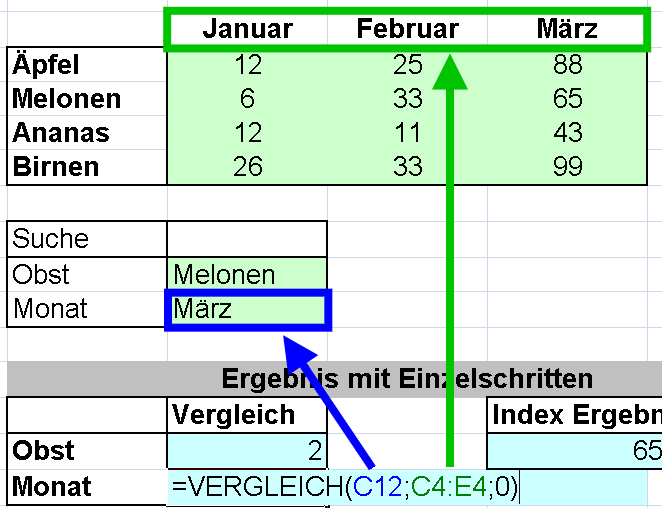
\includegraphics[width=5cm]{images/matrix_maerz}
		\label{fig:matrixmaerz	}} , {März}
]

Genauso wird nun beim Monat verfahren, dessen Spalte in  \xlc{C17} ermittelt wird.
$ \text{ {\stmt{=VERGLEICH(C12; C4:E4; 0)}}} $
%
Das Ergebnis ist, dass der Monat März in der dritten Zelle des Bereiches \xlc{C4:E4} zu finden ist.
\end{figwindow} 
\vspace{2.5cm}
%
Nachdem nun sowohl die Spalte als auch die Zeile des Datenbereiches bekannt ist, kann man mit der Funktion \stmt{INDEX} den gesuchten Wert aus der Matrix ermitteln.
%
$$ \text{\stmt{=INDEX(\syntax{Matrix}; \syntax{Zeile}; \syntax{Spalte})}} $$%
%
Überträgt man nun die ermittelte Zeile und Spalte in diese Formel, so sieht das Ergebnis so aus
%
$$ \text{\stmt{=INDEX(C5:E8; C16; C17)}} $$
%
Die Zwischenschritte werden normalerweise nicht gemacht, sondern es wird die komplette Formel in einer Zelle verwendet. Dann sieht das Ergebnis so wie in \stmt{D21} aus
%
$$ \text{\stmt{=INDEX(C5:E8;VERGLEICH(C11;B5:B8;0);VERGLEICH(C12;C4:E4;0))}} $$%
%

\pagebreak
\subsection{\stmt{SVERWEIS}}


$$ \text{\stmt{SVERWEIS( \syntax{Suchkriterium}; \syntax{Matrix}; \syntax{Spaltenindex}; [\syntax{Bereichsverweis}]} )}$$
Diese Funktion ist eine Art Kombination aus \stmt{VERGLEICH} und \stmt{INDEX} in der Matrixversion. Sie sucht ähnlich wie \stmt{VERGLEICH} innerhalb einer Spalte einen Suchwert und gibt aus einer Matrix den Wert im Schnittpunkt der so gefundenen Zeile mit einer eingegebenen Spaltenzahl zurück.



\begin{description}[labelindent=0cm, leftmargin=3.5cm, font=\mdseries, labelwidth=3.5cm,style=nextline]
\item[\syntax{Suchkriterium}] Dieser Wert wird in der in der ersten Spalte, also die sich ganz links befindet, der Suchmatrix gesucht. Genauso wie bei der \stmt{VERGLEICH} Funktion gibt es einen \stmt{\#NV} Fehler, wenn der Suchwert kleiner als der kleinste Wert in der Suchspalte ist.
\item[\syntax{Matrix}] Ein Zellbezug von mindestens zwei Spalten
\item[\syntax{Spaltenindex}] Eine Ganzzahl, welche jene Spalte der Matrix angibt, deren Wert zurückgegeben werden soll. Wenn eine Spalte < 1 gewählt wird, gibt es den Fehler \stmt{\#Wert!}, ist die gewünschte Spalte größer als die Spaltenzahl der Matrix, dann gibt es einen Fehler \stmt{\#Bezug!}.
\item[\syntax{Bereichsverweis}] %
	\begin{description}[labelindent=0cm, leftmargin=3cm, font=\mdseries, labelwidth=3cm,style=nextline]
	\item[\stmt{WAHR} (default)] Sucht nach dem größtem Wert, der kleiner oder gleich dem Suchkriterium ist. Die erste Spalte der Suchmatrix muss aufsteigend sortiert sein.
	\item[\stmt{FALSCH}] Sucht eine genaue ÜBereinstummung. Hier muss die erste Spalte der Matrix \textit{nicht} sortiert sein.
	\end{description}


\end{description}

Nehmen wir an, dass Kunden auf Grund ihrer Umsätze am Ende des Jahres einen Rabatt bekommt. Es wird also für jeden Kunden einzeln in der Rabatttabelle, welche hier die Matrix ist, nachgesehen, welchen Rabatt der Kunde bekommt. 

\pagebreak
	\begin{figure}[H]
		\centering
%			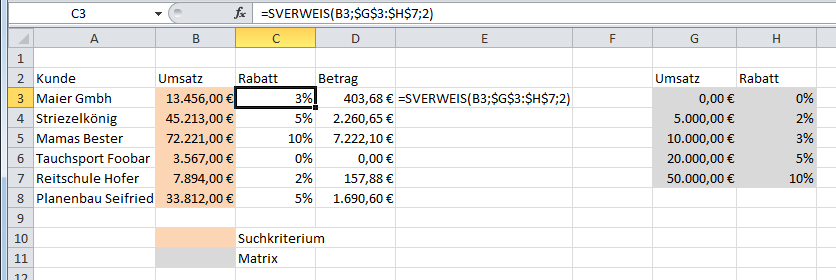
\includegraphics[width=12cm]{images/sverweis_b}
			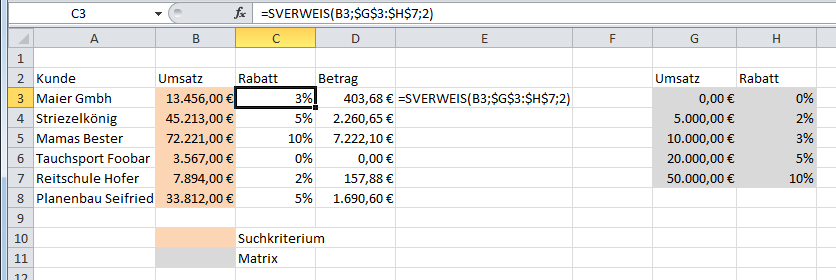
\includegraphics[scale=0.7]{images/sverweis_b}
		\caption{\stmt{SVERWEIS} zur Rabattfindung}
		\label{fig:sverweis}
	\end{figure}
Bei der Reitschule Hofer beträgt der Jahresumsatz 7.894 Euro. Dieser Wert wird herangezogen, um in der Umsatzspalte der Matrix, dem Bereich \xlc{F3:G7}, die Zeile zu finden die größer gleich dem Wert in der Zeile, aber kleiner als der Wert in der nächsten Zeile ist. 7.894 ist größer als 5.000, aber kleiner als 10.000. Daher ist diese Zeile die gesuchte. Nun wollen wir nur den Wert aus der zweiten Spalte, die ja den Rabattbetrag festlegt.




\begin{lightbulbbox}
Man kann sich die Funktion des \stmt{SVERWEIS} ganz einfach durch "`Was suche ich wo und die wievielte Spalte will ich als Ergebnis haben."' merken.
\end{lightbulbbox}


\begin{lightbulbbox}
Beim Verwenden von \stmt{SVERWEIS} wird gerne übersehen, dass man den Matrixbereich in der Formel fixieren sollte. Also statt \xlc{F4:G7} sollte \xlc{\$F\$4:\$G\$7} verwendet werden. Dadurch wird der Matrixbereich beim Kopieren der Formel in andere Zellen nicht verändert.
\end{lightbulbbox}


\subsection{\stmt{WVERWEIS}}


Der \stmt{WVERWEIS} funktioniert genauso wie der \stmt{SVERWEIS}, nur dass die Matrix nicht zeilenorientiert, sondern spaltenorientiert augebaut ist.


$$ \text{\stmt{SVERWEIS( \syntax{Suchkriterium}; \syntax{Matrix}; \syntax{Zeilenindex}; [\syntax{Bereichsverweis}]} )}$$

Das Beispiel aus dem Abschnitt mit dem \stmt{SVERWEIS} würde also so aussehen.
	\begin{figure}[H]
		\centering
%			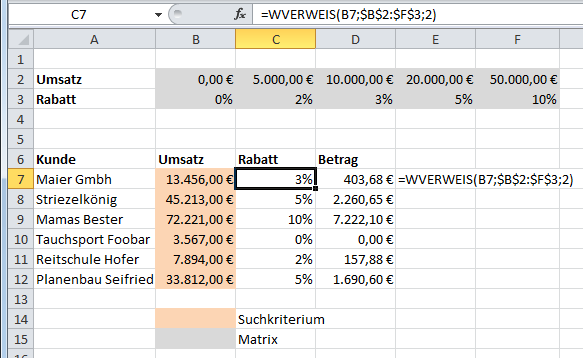
\includegraphics[width=12cm]{images/wverweis_b}
			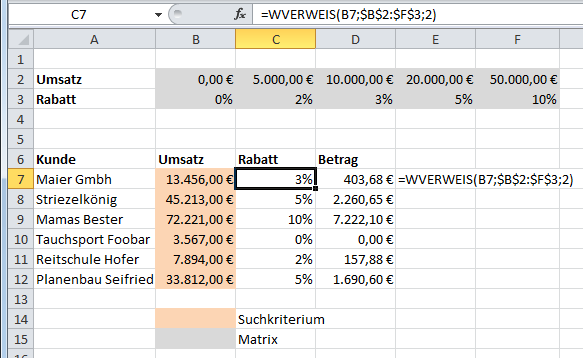
\includegraphics[scale=0.7]{images/wverweis_b}
		\caption{\stmt{WVERWEIS} zur Rabattfindung}
		\label{fig:wverweis}
	\end{figure}
\section{Daten filtern}

Aus Tabellen (Listen) können Daten nach bestimmten Kriterien gefiltert werden. Alle Zeilen, welche nicht dem Filterkriterium entsprechen werden dabei ausgeblendet.

Wenden Sie mehrere Filter an, so ist deren Wirkung kumulativ. Das bedeutet, dass der zweite Filter nur noch mit den Daten arbeitet, welche das erste Filter bereitstellt.

Generell ist zu beachten, dass in den Spalten immer nur ein Datentyp vorkommen darf, wie es auch relationale Datenbanken vorschreiben. Also sollen in einer Spalte z.B. immer nur numerische Werte oder Datumswerte vorkommen. Es soll also nicht sein, dass numerische mit nichtnumerischen Werten gemischt werden. Das Autofilter bietet nämlich vom Datentyp abhängige Filter automatisch an. Werden in einer Spalte gemischte Datentypen verwendet, dann wird das Filter für den am häufigsten vorkommenden Datentyp angeboten. 

Wird ein Filter auf eine Spalte angewendet,  für die bereits ein Filter existiert, wird der alte Filter automatisch gelöscht.


Grundsätzlich gibt es in Excel zwei verschiedene Filterarten
\begin{itemize}
	\smallitemize
	\item Autofilter
	\item Spezialfilter
\end{itemize}


\subsection{Autofilter}

\enlargethispage{1cm}
Bevor man das Autofilter einschaltet, sollte man eine Zelle im Datenbereich auswählen. Excel kann dann, wenn man die Überschriften anders als die Datenspalten formatiert hat, automatisch den kompletten Datenbereich auswählen. Danach wählt man \menu[,]{Daten, Sortieren und Filtern, Filter}.
	\begin{figure}[H]
		\centering
%		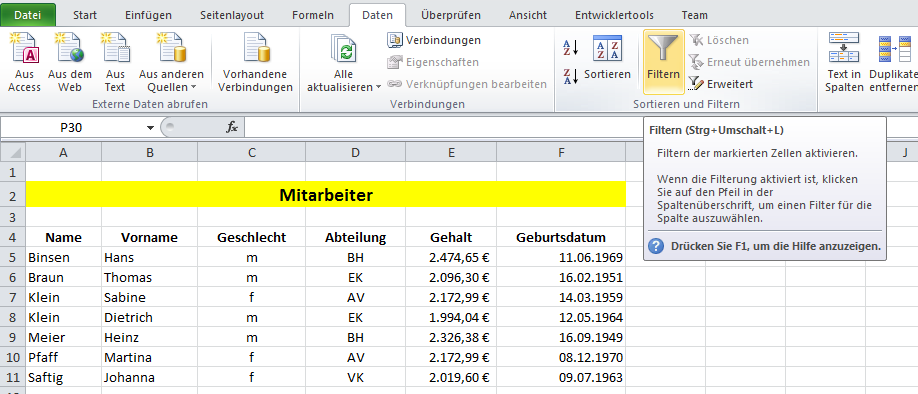
\includegraphics[width=12cm]{images/autofilter_raw.png}
			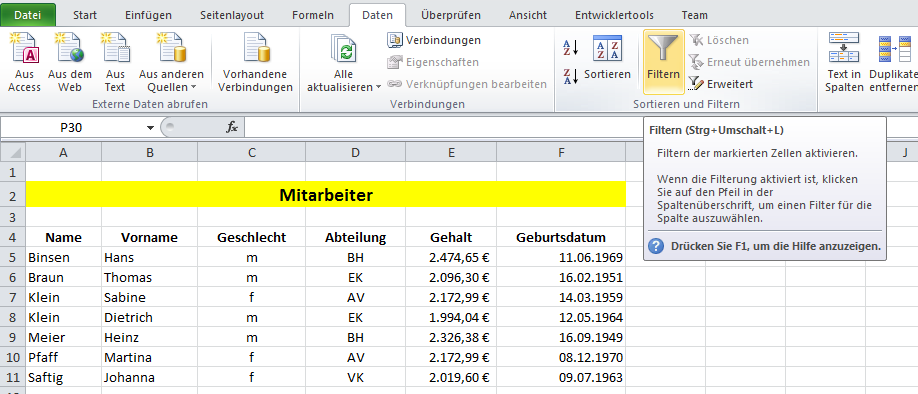
\includegraphics[scale=0.7]{images/autofilter_raw.png}
		\caption{Autofilter aus dem Menü auswählen}
		\label{fig:autofilterMenu}
	\end{figure}%
	\vspace{-1em}
Ist das Autofilter aktiviert, wird neben den Spaltenüberschriften ein kleines Dreieck für die Auswahl der Eingrenzungskriterien angezeigt und das Symbol im Ribbon wird aktiviert angezeigt.
	\begin{figure}[H]
		\centering
	%		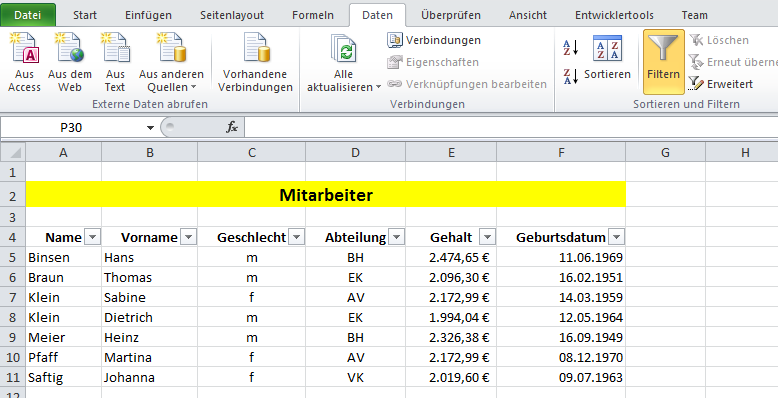
\includegraphics[width=12cm]{images/autofilter_on}
			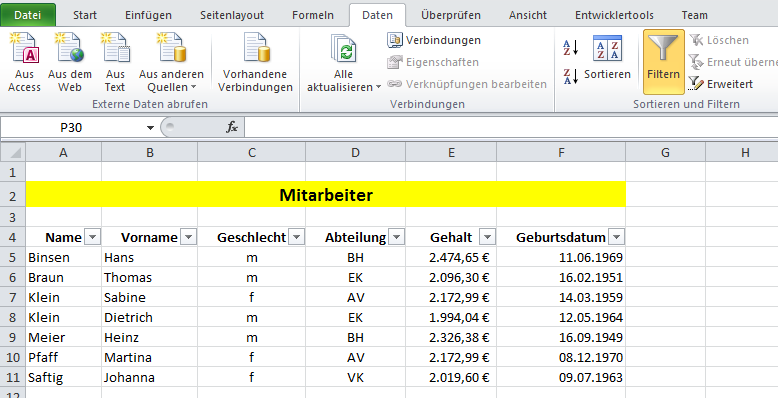
\includegraphics[scale=0.7]{images/autofilter_on}
		\caption{Eingeschaltetes Autofilter}
		\label{fig:autofilterOn}
	\end{figure}
Autofilter liefern schnell Ergebnisse, wenn es sich um einfache unkomplizierte Bedingungen handelt. Je nach Datentyp in einer Spalte zeigt das Autofilter unterschiedliche Optionen an.
	\begin{figure}[H]
		%\captionsetup[subfigure]{labelformat=empty}
   	\centering
		\subfloat[Autofilter bei Datumsspalten]{%
			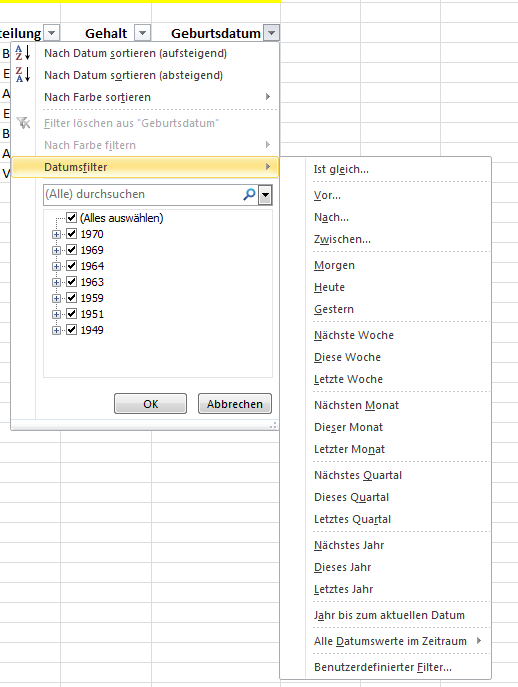
\includegraphics[width=5cm]{images/autofilter_datumsfilter}
			\label{fig:flowlayout1}
		}%
		\quad
		\subfloat[Autofilter bei Zahlenspalten]{%
			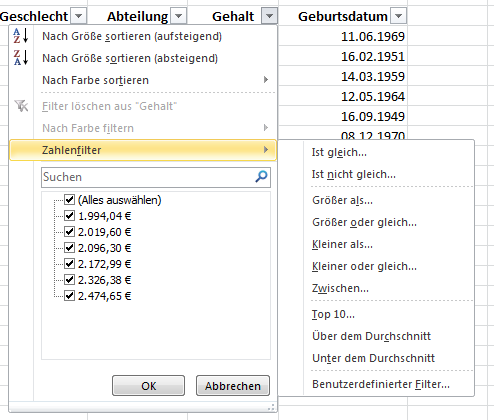
\includegraphics[width=5cm]{images/autofilter_zahlenfilter}
			\label{fig:flowlayout2}
		}%
		\quad
		\subfloat[Autofilter bei Textspalten]{%
			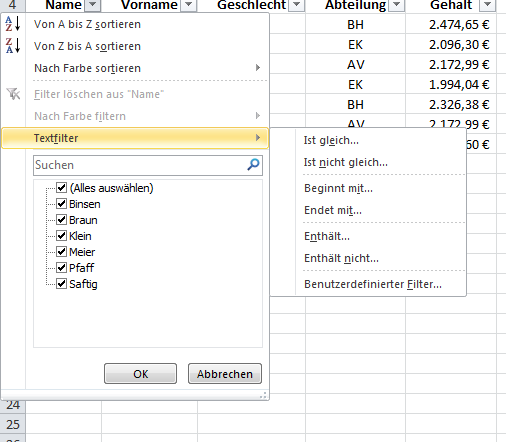
\includegraphics[width=5cm]{images/autofilter_textfilter}
			\label{fig:flowlayout3}
		}%
		\caption{Inhaltsabhängige Filtermöglichkeiten}
	\end{figure}
	
	
\subsection{\stmt{TEILERGEBNIS}}
	
Zeilen, welche nicht vom Filter betroffen sind, werden einfach ausgeblendet. Häufig ist man aber nicht an den einzelnen Datensätzen interessiert, sondern an aggregierten, d.h. zusammengefassten, Werten. Dies kann eine Summe, ein Durchschnitt oder Maximum sein. Die von Excel bekannten Funktionen nehmen allerdings keine Rücksicht auf ausgeblendete Zeilen, also sind sie für diese Aufgabenstellung nicht verwendbar. Um aggregierte Werte zu erhalten wird daher die \stmt{TEILERGEBNIS} Funktion verwendet.
$$ \text{\stmt{TEILERGEBNIS( \syntax{Funktion}; \syntax{Bezug}; \ldots; \syntax{[Bezug\_n]})}} $$%
%
Die \syntax{Funktion} gibt die Art der Aggregation an. Eine Auflistung der Aggregatsfunktionen mit ihren Funktionsnummern zeigt die \tabref{tab:teilergebnis}.
\begin{table}[H]
	\centering
		\begin{tabular}{@{}lcc@{}}
			\toprule  & \multicolumn{2}{c}{\textbf{Funktion}}\\
			 & \parbox[t]{5cm}{\centering berücksichtigt\\ausgeblendeten Zellen} & \parbox[t]{5cm}{ \centering ignoriert\\ausgeblendete Zellen}\\
			\midrule Mittelwert & 1 & 101\\
			Anzahl & 2 & 102 \\
			Anzahl2 & 3 & 103\\
			Max & 4 & 104 \\
			Min & 5 & 105 \\
			Produkt & 6 & 106 \\
			Stabw & 7 & 107 \\
			Stabwn & 8 & 108 \\
			Summe & 9 & 109 \\
			Varianz & 10 & 110 \\
			Varianzen & 11 & 111\\
		\end{tabular}
	\caption{Funktionsnummern der Aggregatfunktionen}
	\label{tab:teilergebnis}
\end{table}%
\vspace{-1em}
In der \figref{fig:teilergebnis} kann man sehen, wie sich ausgeblendete Zeilen auswirken. In der Tabelle ist die dritte Zeile ausgeblendet und die Funktion 109 liefert daher den um den Zellwert reduzierten Summenwert gegenüber der Funktion 9. In diesem Beispiel ist der Zellinhalt 3, die Summe also 12. \figref{fig:teilergebnisbeispiel} zeigt weiters die Gehaltssumme der Abteilung BH mit Hilfe des Autofilter und \stmt{TEILERGEBNIS}.
\enlargethispage{1cm}
	\begin{figure}[H]
		\centering
%			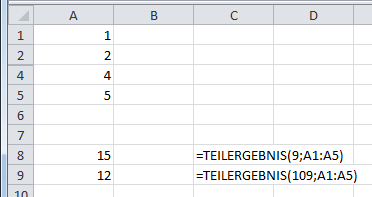
\includegraphics[width=8cm]{images/teilergebnis}
			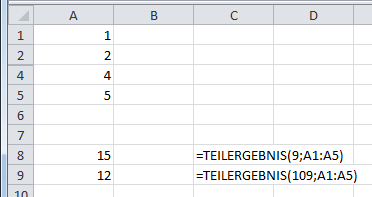
\includegraphics[scale=0.7]{images/teilergebnis}
		\caption{\stmt{TEILERGEBNIS} und ausgeblendete Zeilen}
		\label{fig:teilergebnis}
	\end{figure}%
%\pagebreak
\vspace{-1em}
%Für ein weiteres Beispiel wollen wir die Gehaltssumme der Abteilung BH mit Hilfe des Autofilter und \stmt{TEILERGEBNIS} ermitteln. 
	\begin{figure}[H]
		\centering
%			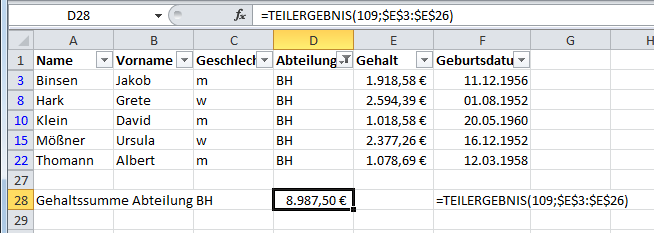
\includegraphics[width=8cm]{images/teilergebnis-beispiel}
			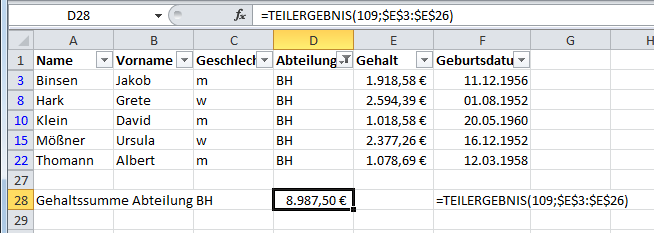
\includegraphics[scale=0.7]{images/teilergebnis-beispiel}
		\caption{Gehaltssumme der Abteilung BH mit \stmt{TEILERGEBNIS} }
		\label{fig:teilergebnisbeispiel}
	\end{figure}

\begin{lightbulbbox}
Es ist wichtig, dass alle Auswertungen, wie Berechnungen, Ergebnisse oder kopierte Ergebnisse von Spezialfiltern entweder oberhalb, unterhalb der Datengrundlage oder auf einem eigenen Tabellenblatt plaziert wird.

Es kann sonst passieren, dass durch das Filter diese Ergbnisse mit ausgeblendet werden und daher nicht mehr sichtbar sind!

\end{lightbulbbox}

%\pagebreak
\subsection{Spezialfilter}
\enlargethispage{1cm}
Mit dem Autofilter stoßen wir recht bald an die Grenzen der Übersichtlichkeit und Flexibilität. Das Spezialfilter ist ein mächtigeres Autofilter, bei dem die Filterkriterien explizit angeführt werden müssen.


	\begin{figure}[H]
		\centering
%			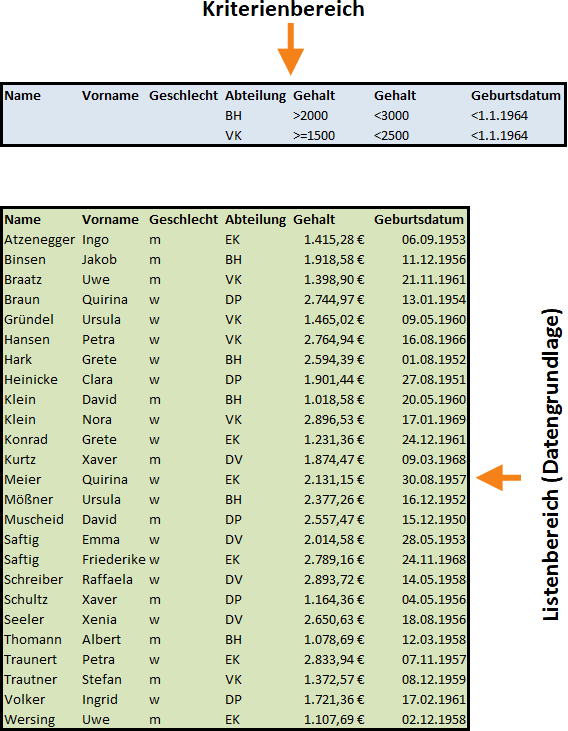
\includegraphics[width=8cm]{images/spezialfilter}
			\includegraphics[scale=0.7]{images/spezialfilter}
		\caption{Spezialfilter mit Datenbereich und Kriterienbereich }
		\label{fig:spezialfilter}
	\end{figure}
	
	
\subsection{Spezialfilter Kriterienbereich}

Der Kriterienberreich des Spezialfilters wird benötigt, um Regeln zu erstellen, welche Datensätze gefiltert werden sollen

	\begin{figure}[H]
		\centering
%			\includegraphics[width=12cm]{images/spezialfilter-kriterienbereich}
			\includegraphics[scale=0.7]{images/spezialfilter-kriterienbereich}
		\caption{Spezialfilter Kriterienbereich }
		\label{fig:spezialfilterKriterienbereich}
	\end{figure}
	
Wie funktioniert nun das Filtern mit einem Spezialfilter? Vom Listenbereich kopiert man jene Überschriften, nach deren Wertinhalt gefiltert werden soll. Diese Überschriften kopiert man in einen Bereich oberhalb oder unterhalb des Listenbereiches. Soll in einer Spalte nach einem Bereich gefiltert werden, so muss die Überschrift zwei Mal abgebildet werden. Einmal für den Vergleich für die untere Grenze und ein Mal für die obere Grenze.
	
In oben gezeigtem Beispiel werden alle MitarbeiterInnen gefiltert, welche vor dem 1.1.1964 geboren wurden, in der Abteilung BH arbeiten und ein Gehalt von über 2.000 und unter 3.000 Euro erhalten. Des weiteren werden auch Datensätze von Mitarbeitenden angezeigt, welche vor dem 1.1.1964 geboren wurden, in der Abteilung VK arbeiten und ein Gehalt von mindestens 1.500 und unter 2.500 Euro verdienen.

\begin{lightbulbbox}
Merke:
\begin{itemize}
	\smallitemize
	\item Alle Spalten in einer Kriterienzeile sind \textit{UND} verknüpft
	\item Alle Zeilen des Kriterienbereiches sind \textit{ODER} verknüpft
\end{itemize}
\end{lightbulbbox}
%
\begin{lightbulbbox}
Es ist immer besser, wenn man die Spaltenüberschriften kopiert und nicht tippt, da sich Tippfehler einschleichen können. Tippfehler bewirken nämlich nicht, dass das Filtern nicht funktioniert, sondern man erhält ein berechnetes Feld, welches in \kapref{sec:berechneteFelder} noch näher erklärt wird.
\end{lightbulbbox}
	
\subsection{Spezialfilter Vergleichsoperationen}
	
\FloatBarrier
%\begin{figure*}[H]
\begin{table}[H]
	\centering
		\begin{tabular}{@{}p{4cm}p{2cm}@{}}
			\toprule \multicolumn{2}{c}{ \parbox[t]{6cm}{\centering \textbf{Vergleichsoperatoren für \\numerische- oder Datumswerte}}}\\
			\midrule ist gleich 20 &  $=20$\\
			größer $20$ & $>20$  \\
			größer gleich $20$ & $>=20$  \\
			kleiner $20$ & $<20$  \\
			kleiner gleich $20$ & $<=20$  \\
			ungleich $20$ & $<>20$\\
		\end{tabular}
	\caption{Numerische und Datumsvergleichsoperatoren}
\end{table}
%\end{figure*}
\vspace{-1em}
\FloatBarrier
%\begin{figure*}
\begin{table}[H]
	\centering
		\begin{tabular}{@{}p{9cm}p{6cm}@{}}
			\toprule \multicolumn{2}{c}{ \parbox[t]{9cm}{\centering \textbf{Vergleichsoperatoren für \\alphanumerische Werte}}}\\
			\midrule alle die mit "`Klein"' beginnen &  Klein\\
			alle die im Text "`Klein"' beinhalten & *Klein* \\
			 \parbox[t]{8cm}{alle Werte die mit A, B oder C beginnen\\ (D ist ausgeschlossen)}  & $<D$ \\
			 \parbox[t]{8cm}{alle Werte die mit X, Y oder Z beginnen\\ (Xx ist eingeschlossen)}  & $>X$ \\
			 beliebiges Zeichen an einer bestimmten Stelle & $?$ \\
			 kein, ein oder mehrere beliebige Zeichen & * \\
			 "`*"' als normales Zeichen & \~{}* \\
			 "`?"' als normales Zeichen & \~{}? \\
			 "`\~{}"' als normales Zeichen & \~{}\~{} \\
			 \parbox[t]{9cm}{Suchen nach exaktem Wert unter Berücksichtigung\\\quad der Groß- und Kleinschreibung} & =\stmt{IDENTISCH}(A5; "Klein"') \\
			 Suche nach leerer Zelle &  =\upquote{}\\
		\end{tabular}
	\caption{Alphanumerische Vergleichsoperatoren}
\end{table}
%\end{figure*}
\FloatBarrier

\subsection{Spezialfilter aktivieren}

Bevor man das Spezialfilter aktiviert, sollte man sich überlegen, wo die gefilterten Daten angezeigt werden sollen. Es gibt hierbei drei Möglichkeiten.
\begin{itemize}
	\smallitemize	
	\item An der gleichen Stelle wie die Datengrundlage anzeigen
	\item Am selben Tabellenblatt wie die Datengrundlage anzeichen, aber an anderer Stelle
	\item Auf einem anderen Tabellenblatt anzeigen
\end{itemize}

Die Vorgehensweise ist dabei identisch, es wird mit \menu[,]{Daten, Sortieren und Filtern, Erweitert} aufgerufen
	\begin{figure}[H]
		\centering
%			\includegraphics[width=12cm]{images/spezialfilter-menu}
			\includegraphics[scale=0.65]{images/spezialfilter-menu}
		\caption{Spezialfilter Menü}
		\label{fig:spezialfilterMenu}
	\end{figure}
	\vspace{-1em}
Danach wird in der Dialogbox entweder \textit{An gleicher Stelle filtern} gewählt, wenn die Daten im Listenbereich angezeigt werden sollen. Will man dagegen die Daten in einem anderen Bereich eines Arbeitsblattes oder in einem anderen Arbeitsblatt anzeigen, dann muss man \textit{An eine adere Stelle kopieren auswählen}
\enlargethispage{1cm}
	\begin{figure}[H]
		\centering
%			\includegraphics[width=12cm]{images/spezialfilter-dialogbox}
			\includegraphics[scale=0.65]{images/spezialfilter-dialogbox}
		\caption{Spezialfilter aktivieren}
		\label{fig:spezialfilterAktivieren}
	\end{figure}

\begin{lightbulbbox}
Will man die gefilterten Daten am gleich Datenblatt haben, so empfielt es sich, dass man vor dem Aufrufen des Spezialfilters den Cursor innerhalb des Datenbereiches setzt, da dieser dann automatisch von Excel erkannt und ausgewählt wird.
\end{lightbulbbox}
%\pagebreak
\begin{lightbulbbox}
Eine besondere Falle liefert Excel, wenn das Ergebnis auf ein anderes Tabellenblatt kopiert werden soll. Man muss \textit{immer} zwingend von dem Tabellenblatt ausgehen, auf dem die gefilterten Daten angezeigt werden. Macht man dies nicht, so liefert Excel die Fehlermeldung%
	\begin{figure}[H]
	%\vspace{2em}
		\centering
%			\includegraphics[width=8cm]{images/spezialfilter-fehler2010}
			\includegraphics[scale=0.7]{images/spezialfilter-fehler2010}
		\caption{Spezialfilter Fehlermeldung}
		\label{fig:spezialfilterFehlermeldung}
	\end{figure}
\end{lightbulbbox}


\subsection{Spezialfilter mit berechneten Feldern}
\label{sec:berechneteFelder}

Eine Besonderheit im Kriterienbereich sind berechnete Felder. Im Gegensatz zu normalen Kriterien wird hier nicht direkt eine Spalte der Datengrundlage mit einem Wert verglichen, sondern der zu vergleichende Wert wird über eine Formel bestimmt. Berechnete Felder kommen zum Einsatz, wenn an der Datengrundlage nichts geändert werden darf oder kann.

Nehmen wir als Beispiel, dass wr alle MitarbeiterInnen der Abteilung BH herausfinden wollen, welche ein Jahreseinkommen von über 30.000\texteuro\ haben.  Das Jahreseinkommen ist das 14-fache des Monatsgehaltes plus der Zulage. 

Bei berechneten Feldern sind folgende Dinge zu beachten
\begin{itemize}
	\smallitemize
	\item Die Überschrift im Kriterienbereich darf  \textit{niemals} mit einer der Überschriften der Datengrundlage übereinstimmen. Der Grund liegt darin, dass es sich hier um eine "`künstliche"' Spalte handelt.
	\item Berechnete Felder beginnen immer mit $=$, da es sich um eine Formel handelt
	\item Die Formel in berechneten Feldern muss immer \stmt{WAHR} oder \stmt{FALSCH} ergeben
	\item Wenn bei der Berechnung Werte der Datengrundlage herangezogen werden, muss \textit{immer} der Wert aus der \textit{ersten} Zeile der Datengrundlage genommen werden.
\end{itemize}
\enlargethispage{2cm}
Wie wird das nun in der zu lösenden Aufgabe umgesetzt?
	\begin{figure}[H]
		\centering
%			\includegraphics[width=10cm]{images/spezialfilter-berechnet1}
			\includegraphics[scale=0.7]{images/spezialfilter-berechnet1}
		\caption{Spezialfilter mit berechnetem Feld}
		\label{fig:spezialfilterBerechnetesFeld}
	\end{figure}
	
	
	
Die Formel für die Berechnung lautet $14*Gehalt+Zulage$. Mit dieser Formel soll jede Zeile des Listenbereichs verglichen werden. Ist das Ergebnis größer als 30.000, dann soll diese Zeile im Ergebnis aufscheinen. Die erste Zeile des Listenbereiches ist die Zeile 5, also muss diese für den Vergleich herangezogen werden. Das Kriterium lautet daher
\begin{equation}
	\text{\stmt{= 14 * E5 + G5 > 30000}}
\end{equation}
wie auch in der Abbildung ersichtlich ist.


\section{Datenbankfunktionen}

Datenbankfunktionen ermöglichen eine aggregierte Auswertung großer Listen mit komplexen Filterkriterien, die identisch aufgebaut sind, wie jene des Spezialfilter Kriterienbereiches. Deswegen sie sehr oft in Zusammenhang mit dem Spezialfilter vwerwendet, da sie neben dem reinen Filtern von Datensätzen auch wichtige Informationen wie Maximum Minimum oder Summe eines gefilterten Datenbereiches liefern. Im Prinzip kann da auch die bereits bekannte \stmt{TEILERGEBNIS} Funktion, welche aber den Nachteil hat, dass bei geänderten Bedingungen \textit{keine} Neuberechnung stattfindet.

Die Datenbankfunktionen sind

\begin{multicols}{2}
	\begin{itemize}
	\smallitemize
    	\item \stmt{DBANZAHL}
	    \item \stmt{DBANZAHL2}
    	\item \stmt{DBMAX}
    	\item \stmt{DBMIN}
	    \item \stmt{DBPRODUKT}
    	\item \stmt{DBMITTELWERT}
    	\item \stmt{DBSTDABWN}
	\end{itemize}
\end{multicols}

Die Anzahl und der Aufbau der Parameter der Datenbankfunktionen sind bei alles oben genannten gleich, daher folgt hier die Beschreibung anhand von \stmt{DBSUMME}.
$$ \text{\stmt{DBSUMME( \syntax{Datenbank}; \syntax{Datenbankfeld}; \syntax{Suchkriterien})}} $$
\pagebreak
\begin{description}[labelindent=0cm, leftmargin=3.5cm, font=\mdseries, labelwidth=3cm,style=nextline]
\smallitemize
\item[\syntax{Datenbank}]Ist die Datengrundlage \textit{inklusive} der Überschriften
\item[\syntax{Datenbankfeld}] Ist die Spalte an der die Datenbankfunktion durchgeführt werden soll. Wichtig ist hier, dass die Überschrift der Spalte ausgewählt wird.
\item[\syntax{Suchkriterien}] Diese bestimmen, genauso wie beim Kriterienbereich des Spezialfilters, welche Datensätze für die Aggregatfunktion herangezogen werden sollen. Wie auch beim Spezialfilter werden im Kriterienbereich Spalten \stmt{UND} verknüpft und Zeilen \stmt{ODER} verknüpft.
\end{description}
%
%\pagebreak
Als Beispiel will ein Controller folgende Dinge in einem Unternehmen wissen
\begin{itemize}
	\smallitemize
	\item wie viele Mitarbeiter arbeiten in der Abteilung VK,
	\item wie viele Mitarbeiter sind davon über 50 Jahre alt,
	\item die Gehaltssumme der Abteilung VK
\end{itemize}

	\begin{figure}[H]
		\centering
%			\includegraphics[width=10cm]{images/datenbankfunktion}
			\includegraphics[scale=0.7]{images/datenbankfunktion}
		\caption{Datenbankfunktionen}
		\label{fig:datenbankfunktionen}
	\end{figure}

Will der Controller nun statt der Abteilung VK jetzt die Abteilung EK wissen, braucht er nur in der Zelle \xlc{C2} den Wert \upquote{VK} auf \upquote{EK} ändern und erhält sofort das Ergebnis.


\section{Erweiterte \stmt{WENN} Funktionen}

\subsection{\stmt{SUMMEWENN} Funktion}

Mit dieser Funktion kann man in Zellbereichen numerische Werte addieren, die bestimmten Bedingungen in gleichen oder anderen Zellbereichen unterworfen sind.%
$$ \text{\stmt{WENN(\syntax{Bereich}; \syntax{Suchkriterien}; \syntax{SUMME\_BEREICH})}}$$%
%
Das folgende Beispiel zeigt die Umsätze in Abhängigkeit der Kategorie%
	\begin{figure}[H]
		\centering
%			\includegraphics[width=10cm]{images/summewenn}
			\includegraphics[scale=0.7]{images/summewenn}
		\caption{\stmt{SUMMEWENN} Funktion}
		\label{fig:summewenn}
	\end{figure}

\subsection{\stmt{SUMMEWENNS} Funktion}

Bei dieser Funktion kann man Werte addieren, welche anhand von bis zu 127 Kriterien gefilter wurden

$$ \text{\stmt{WENN(\syntax{Summe\_Bereich}; \syntax{Kriterien\_Bereich1}; \syntax{Kriterien1}; \ldots)}}$$%
%
\begin{description}[labelindent=0cm, leftmargin=4cm, font=\mdseries, labelwidth=3cm,style=nextline]
\smallitemize
\item[\syntax{Summe\_Bereich}] Jener Zellbereich, der summiert werden soll.
\item[\syntax{Kriterien\_Bereich1}] Jener Zellbereich, auf den das Kriterium $(n)$ angewendet werden soll.
\item[\syntax{Kriterien1}] Jene Suchbedingung, die auf den Kriterien Bereich $(n)$ angewendet werden soll.
\end{description}

\figref{fig:summewenns} zeigt die Umsätze in Abhängigkeit der Kategorie und eines Zeitraumes%
	\begin{figure}[H]
		\centering
%			\includegraphics[width=14cm]{images/summewenns}
			\includegraphics[scale=0.7]{images/summewenns}
		\caption{\stmt{SUMMEWENNS} Funktion}
		\label{fig:summewenns}
	\end{figure}



\subsection{\stmt{ZÄHLENWENN} Funktion}

Mit dieser Funktion kann man die Anzahl der zutreffenden Zellen zählen, die bestimmten Bedingungen entsprechen.%
$$ \text{\stmt{WENN(\syntax{Bereich}; \syntax{Suchkriterien}; \syntax{SUMME\_BEREICH})}}$$%
%
Das folgende Beispiel zeigt die Umsätze in Abhängigkeit der Kategorie%
	\begin{figure}[H]
		\centering
%			\includegraphics[width=10cm]{images/zaehlenwenn}
			\includegraphics[scale=0.7]{images/zaehlenwenn}
		\caption{\stmt{ZÄHLENWENN} Funktion}
		\label{fig:zaehlenwenn}
	\end{figure}

\subsection{\stmt{ZÄHLENWENNS} Funktion}

Bei dieser Funktion kann man Werte zählen, welche anhand von bis zu 127 Kriterien gefiltert wurden

$$ \text{\stmt{WENN(\syntax{Summe\_Bereich}; \syntax{Kriterien\_Bereich1}; \syntax{Kriterien1}; \ldots)}}$$%
%
\begin{description}[labelindent=0cm, leftmargin=4cm, font=\mdseries, labelwidth=3cm,style=nextline]
\smallitemize
\item[\syntax{Summe\_Bereich}] Jener Zellbereich, der summiert werden soll.
\item[\syntax{Kriterien\_Bereich1}] Jener Zellbereich, auf den das Kriterium $(n)$ angewendet werden soll.
\item[\syntax{Kriterien1}] Jene Suchbedingung, die auf den Kriterien Bereich $(n)$ angewendet werden soll.
\end{description}
\pagebreak
\figref{fig:zaehlenwenns} zeigt die Anzahl von Personen, welche in einem bestimmter Altersbereich sind, Raucher sind und Übergewicht haben%
	\begin{figure}[H]
		\centering
%			\includegraphics[width=14cm]{images/zaehlenwenns}
			\includegraphics[scale=0.7]{images/zaehlenwenns}
		\caption{\stmt{ZAEHLENWENNS} Funktion}
		\label{fig:zaehlenwenns}
	\end{figure}



%\input{chapters/10_Bedingte Formatierung}

%\bibliographystyle{unsrtdin}
%\bibliography{bib/references}



\end{document}